\chapter{Simulaciones}
\lhead{\emph{Simulaciones}}

En este capítulo se presentan las mediciones y ensayos realizados para estudiar y comparar como se comportan ambos métodos de
calibración, clásica y utilizando acoplamientos mútuos.

La configuración de la antena a utilizar para todos los ensayos está especificada en la tabla \ref{tab:configurationUsed} y 
consta de 70 elementos radiantes. Las especificaciones de las propiedades físicas de cada componente están definidas en la 
tabla \ref{tab:configurationOfComponents}.
\begin{table}[H]
  \footnotesize
  \centering
  \begin{tabular}{|c|c|}
	\hline
	\textbf{Componente de Antena} & \textbf{Configuración} \tabularnewline \hline 
	freq &  1275000000 [Hz] \tabularnewline\hline 
	power & 0 [dB] \tabularnewline \hline 
	phase & 0 [deg] \tabularnewline \hline 
	desiredTxPower & 6 [dB] \tabularnewline \hline 
	desiredRxPower & 0 [dB] \tabularnewline \hline 
	quantityRows & 7 \tabularnewline \hline 
	quantityColumns & 10 \tabularnewline \hline 
	verticalSeparation & 0.2 [m] \tabularnewline \hline 
	hotizontalSeparation & 0.2 [m] \tabularnewline \hline 
	componentSequence & [cable1, psc17, cable1, psc15, cable2, psc12, trm, circulator, cable3, rm] \tabularnewline \hline 
  \end{tabular}
  \caption{Configuración de la antena común para todos los ensayos.}
  \label{tab:configurationUsed}
\end{table}
\begin{table}[H]
  \footnotesize
  \centering
  \begin{tabular}{|c|c|c|}
	\hline
	\textbf{Componente de Antena} & \textbf{Cacarcterísticas físicas} & \textbf{Configuración} \tabularnewline \hline 
	\multirow{2}{*}{cable1} &  attenuation [db] & 0.1\tabularnewline \cline{2-3}
	 & length [m] & 0.45\tabularnewline \hline 
	\multirow{2}{*}{cable2} &  attenuation [db] & 0.1\tabularnewline \cline{2-3}
	 & length [m] & 8\tabularnewline \hline 
	\multirow{2}{*}{cable3} &  attenuation [db] & 0.1\tabularnewline \cline{2-3}
	 & length [m] & 0.5\tabularnewline \hline 
	psc17 & outputPorts & 7\tabularnewline \hline
	psc15 & outputPorts & 5\tabularnewline \hline
	psc12 & outputPorts & 2\tabularnewline \hline
	\multirow{2}{*}{TRM} & gain [db] & 10\tabularnewline \cline{2-3}
	 & phaseShift [deg] & 10\tabularnewline \hline 
	circulator & & \tabularnewline \hline 
	RM & & \tabularnewline \hline 
  \end{tabular}
  \caption{Configuración de las propiedades físicas de cada componente de la antena utilizada en todos los ensayos.}
  \label{tab:configurationOfComponents}
\end{table}
La numeración de los elementos tiene un orden de izquierda a derecha y de arriba hacia abajo, de tal forma que el elemnto cero 
es el superior izquierdo de la antena.
\todo{agregar imagen con numeración de elementos radiantes}
Para una mayor claridad, todos los gráficos representan cómo ambos métodos calibran la antena en un estado puntual. No se 
realizaron ensayos utilizando el método montecarlo dado que no se agregaron incertidumbres en el instrumento de medición de las 
distintas señales recibidas de los lazos de calibración.

Todos los ensayos de las siguientes secciones poseen las siguientes característicias:
\begin{itemize}
	\item Se utilizan diferentes apuntamientos de la antena. Los cuales son uniforme, 10 grados en la dirección horizontal y 10 
		grados en la dirección vertical.
	\item Se muestra un gráfico de la potencia y fase transmitida para cada apuntamiento utilizado. En los cuales se observan las
		señales sin calibrar, calibrada e ideal. 
	\item Se grafican los diagramas de antena para los cortes horizontal y vertical de las señales transmitidas sin calibrar, 
		calibradas e ideales.
\end{itemize}


\section{Sin dispersiones}

Los ensayos de esta sección tienen las siguientes caracterísiticas,
\begin{itemize}
	\item Los componentes de antena no tienen ningún prolema de funcionamiento ni hay desadaptaciones.
	\item No hay dispersiones de calibración.
	\item No hay dispersiones en la señal.
\end{itemize}

\subsection{Utilizando la calibración clásica}

En las figuras \ref{fig:nonErrClassical0deg}, \ref{fig:nonErrClassical10degCol} y \ref{fig:nonErrClassical10degRow} se muestran
los resultados de la calibración clásica con una antena sin dispersiones. Se puede apreciar que, si bien la antena tiene un 
comportamiento ideal, las mediciones no son completamente correctas. Dicha dispersión se debe a que el método no abarca la 
totalidad de la antena.


\subsubsection{Apuntamiento uniforme}

Los gráficos de la figura \ref{fig:nonErrClassical0deg} muestran que el calibrador, por no abarcar la totalidad del sistema, no 
puede determinar correctamente ni la ganancia ni fase de la antena. Pero, como estas diferencias entre lo real y estimado son 
iguales para cada elemento, el diagrama resultante mantiene su forma y sus atributos no se modifican, salvo la ganancia total.

La tabla \ref{tab:nonErrClassical0deg} muestra como la ganancia relativa de los lóbulos secundarios con respecto al del lóbulo
principal de cada diagrama se mantienen invariantes e iguales al del diagrama ideal. A su vez se puede observar como la diferencia
de la ganancia del diagrama calibrado disminuye pero no llega a ser igual a cero.
\begin{figure}[H]
	\centering
 	\subfloat[]{
		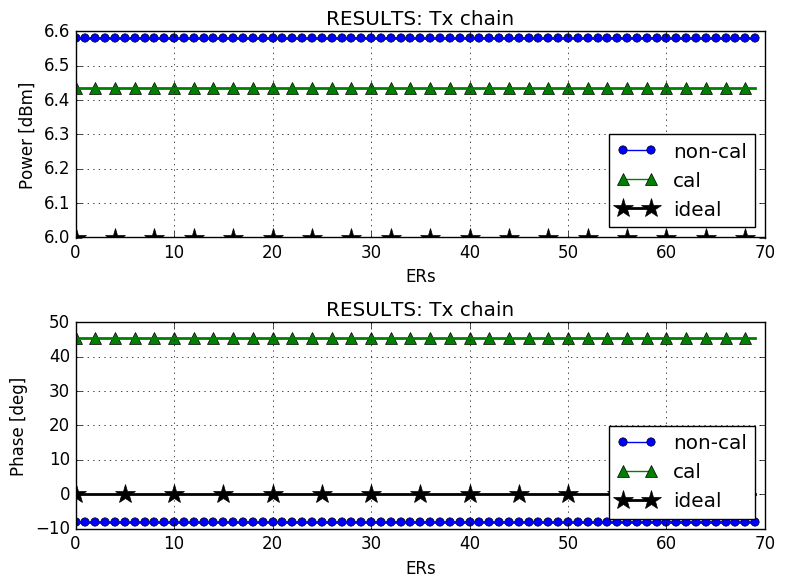
\includegraphics[width=9cm]{gfx/nonErrClassical0deg.png}}

	\subfloat[]{
		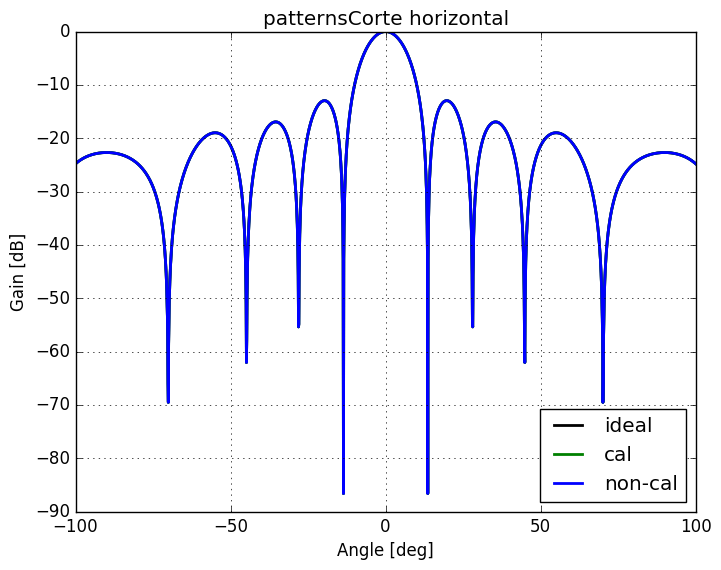
\includegraphics[width=7cm]{gfx/nonErrClassical0degAzCut.png}}
 	\subfloat[]{
		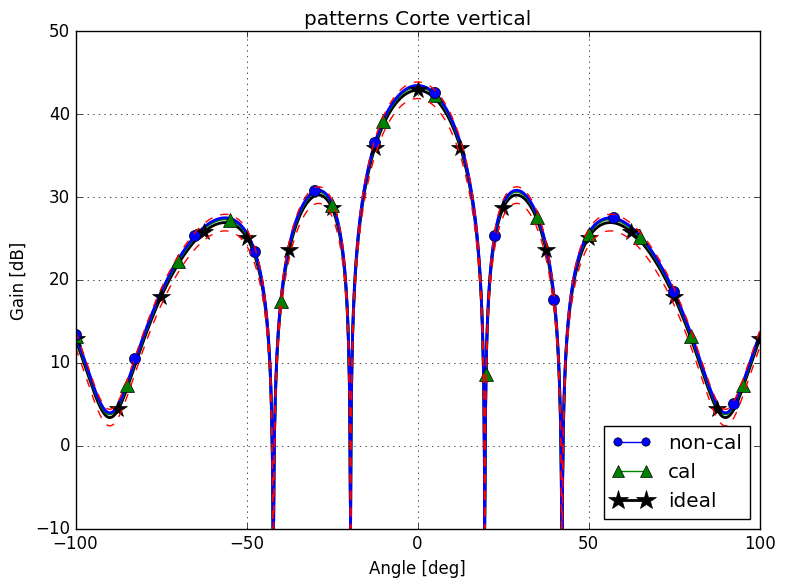
\includegraphics[width=7cm]{gfx/nonErrClassical0degElCut.png}}
	\caption{Correcciones de la señal transmitida utilizando calibración clásica. (a) ganancia y fase transmitida por módulos
		radiantes. (b) corte horizontal del diagrama transmitido y (c) corte vertical del diagrama transmitido.}
	\label{fig:nonErrClassical0deg}
\end{figure}
\begin{table}[H]
  \footnotesize
  \centering
  \begin{tabular}{|c|c|p{2cm}|p{2.5cm}|p{2.5cm}|p{2.5cm}|}
    \cline{2-6}
    \multicolumn{1}{c|}{} & Corte & Ganancia - lóbulo izq. [dBc] & Ganancia - lóbulo central [dB] &
    Ganancia - lóbulo der. [dBc] & Ancho - lóbulo central -3dB \tabularnewline\hline
    \multirow{2}{2cm}{Pat. sin calibrar} & H & 12.97 & 43.48 & 12.97 & 12.0 \tabularnewline\cline{2-6}
     & V & 12.65 & 43.48 & 12.65 & 17.4 \tabularnewline\hline
    \multirow{2}{2cm}{Pat. calibrado} & H & 12.97 & 43.34 & 12.97 & 12.0 \tabularnewline\cline{2-6}
     & V & 12.65 & 43.34 & 12.65 & 17.4 \tabularnewline\hline
    \multirow{2}{2cm}{Pat. ideal} & H & 12.97 & 42.9 & 12.97 & 12.0 \tabularnewline\cline{2-6}
     & V & 12.65 & 42.9 & 12.65 & 17.4 \tabularnewline\hline
    \multirow{2}{2cm}{Dif. sin calibrar} & H & 0.0 & 0.58 & 0.0 & 0.0\tabularnewline\cline{2-6}
     & V & 0.0 & 0.58 & 0.0 & 0.0 \tabularnewline\hline
    \multirow{2}{2cm}{Dif. calibrado} & H & 0.0 & 0.44 & 0.0 & 0.0 \tabularnewline\cline{2-6}
     & V & 0.0 & 0.44 & 0.0 & 0.0 \tabularnewline\hline
  \end{tabular}
  \caption{Propiedades de los patrones calibrados y sin calibrar comparados con el ideal.}
  \label{tab:nonErrClassical0deg}
\end{table}

\subsubsection{Apuntamiento 10 grados en dirección horizontal}

Los gráficos de la figura \ref{fig:nonErrClassical10degCol} muestran que el calibrador, por no abarcar la totalidad del sistema,
no puede determinar correctamente ni la ganancia ni fase de la antena. Pero, como estas diferencias entre lo real y estimado son
iguales para cada elemento, el diagrama resultante no solo se mantiene su forma sino que también apunta en la misma dirección; 
sus atributos no se modifican, salvo la ganancia total.

\begin{figure}[H]
	\centering
 	\subfloat[]{
		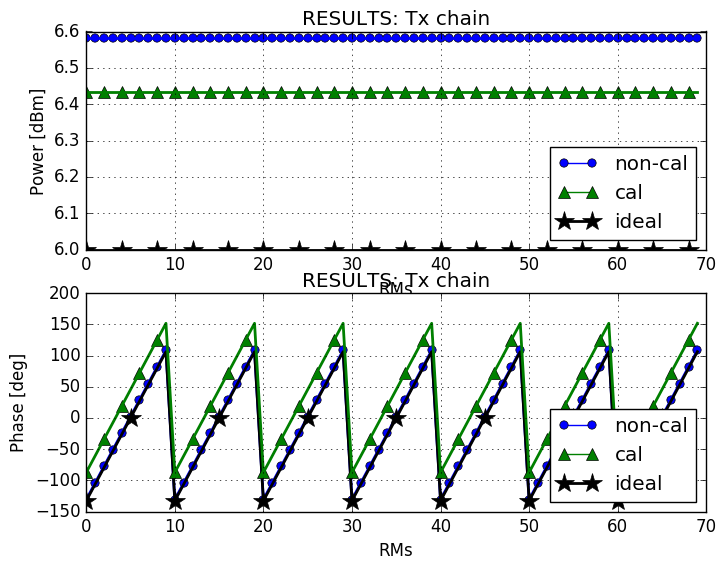
\includegraphics[width=9cm]{gfx/nonErrClassical10degCol.png}}

	\subfloat[]{
		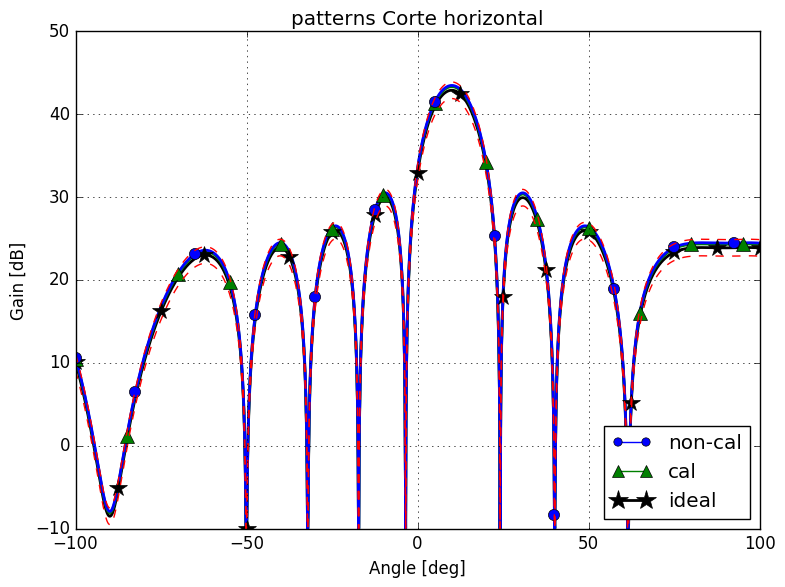
\includegraphics[width=7cm]{gfx/nonErrClassical10degColAzCut.png}}
 	\subfloat[]{
		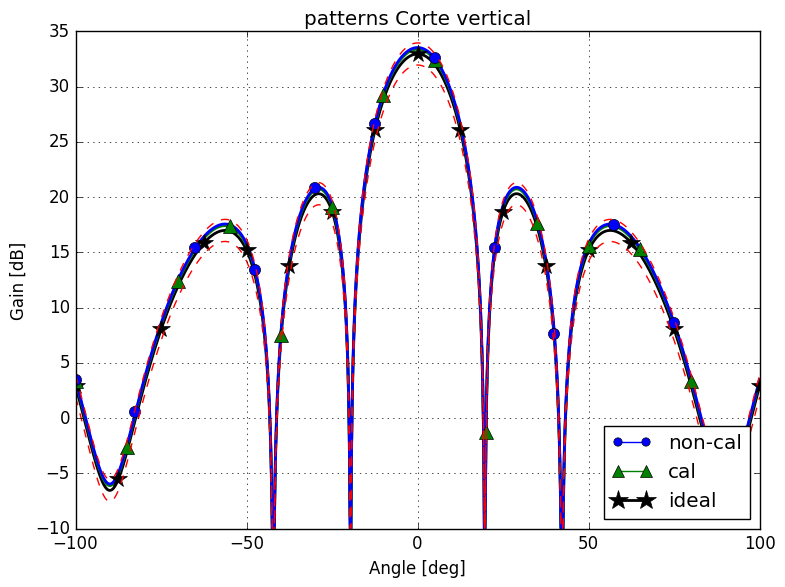
\includegraphics[width=7cm]{gfx/nonErrClassical10degColElCut.png}}
	\caption{Correcciones de la señal transmitida utilizando calibración clásica. (a) ganancia y fase transmitida por módulos
		radiantes. (b) corte horizontal del diagrama transmitido y (c) corte vertical del diagrama transmitido.}
	\label{fig:nonErrClassical10degCol}
\end{figure}

La tabla \ref{tab:nonErrClassical0deg} muestra como la ganancia relativa de los lóbulos secundarios con respecto al del lóbulo
principal de cada diagrama se mantienen invariantes e iguales al del diagrama ideal. A su vez se puede observar como la diferencia
de la ganancia del diagrama calibrado disminuye pero no llega a ser igual a cero.
\begin{table}[H]
  \footnotesize
  \centering
  \begin{tabular}{|c|c|p{2cm}|p{2.5cm}|p{2.5cm}|p{2.5cm}|}
    \cline{2-6}
    \multicolumn{1}{c|}{} & Corte & Ganancia - lóbulo izq. [dBc] & Ganancia - lóbulo central [dB] &
    Ganancia - lóbulo der. [dBc] & Ancho - lóbulo central -3dB \tabularnewline\hline
    \multirow{2}{2cm}{Pat. sin calibrar} & H & 12.97 & 43.48 & 12.97 & 12.4 \tabularnewline\cline{2-6}
     & V & 12.65 & 33.54 & 12.65 & 17.4 \tabularnewline\hline
    \multirow{2}{2cm}{Pat. calibrado} & H & 12.97 & 43.34 & 12.97 & 12.4 \tabularnewline\cline{2-6}
     & V & 12.65 & 33.4 & 12.65 & 17.4 \tabularnewline\hline
    \multirow{2}{2cm}{Pat. ideal} & H & 12.97 & 42.9 & 12.97 & 12.4 \tabularnewline\cline{2-6}
     & V & 12.65 & 32.96 & 12.65 & 17.4 \tabularnewline\hline
    \multirow{2}{2cm}{Dif. sin calibrar} & H & 0.0 & 0.58 & 0.0 & 0.0\tabularnewline\cline{2-6}
     & V & 0.0 & 0.58 & 0.0 & 0.0 \tabularnewline\hline
    \multirow{2}{2cm}{Dif. calibrado} & H & 0.0 & 0.44 & 0.0 & 0.0 \tabularnewline\cline{2-6}
     & V & 0.0 & 0.44 & 0.0 & 0.0 \tabularnewline\hline
  \end{tabular}
  \caption{Propiedades de los patrones calibrados y sin calibrar comparados con el ideal.}
  \label{tab:nonErrClassical10degCol}
\end{table}


\subsubsection{Apuntamiento 10 grados en dirección vertical}

Los gráficos de la figura \ref{fig:nonErrClassical10degRow} muestran que el calibrador, por no abarcar la totalidad del sistema,
no puede determinar correctamente ni la ganancia ni fase de la antena. Pero, como estas diferencias entre lo real y estimado son
iguales para cada elemento, el diagrama resultante no solo se mantiene su forma sino que también apunta en la misma dirección; 
sus atributos no se modifican, salvo la ganancia total.

La tabla \ref{tab:nonErrClassical0deg} muestra como la ganancia relativa de los lóbulos secundarios con respecto al del lóbulo
principal de cada diagrama se mantienen invariantes e iguales al del diagrama ideal. A su vez se puede observar como la diferencia
de la ganancia del diagrama calibrado disminuye pero no llega a ser igual a cero.

\begin{figure}[H]
	\centering
 	\subfloat[]{
		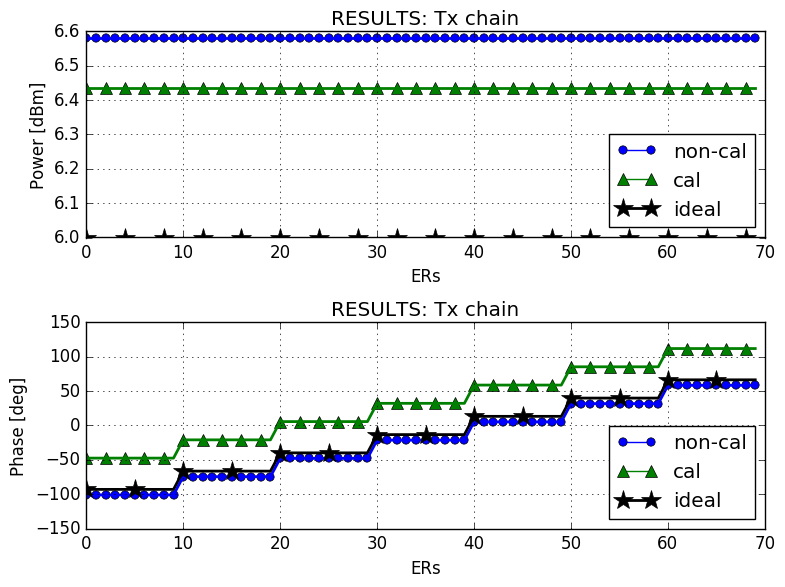
\includegraphics[width=9cm]{gfx/nonErrClassical10degRow.png}}

	\subfloat[]{
		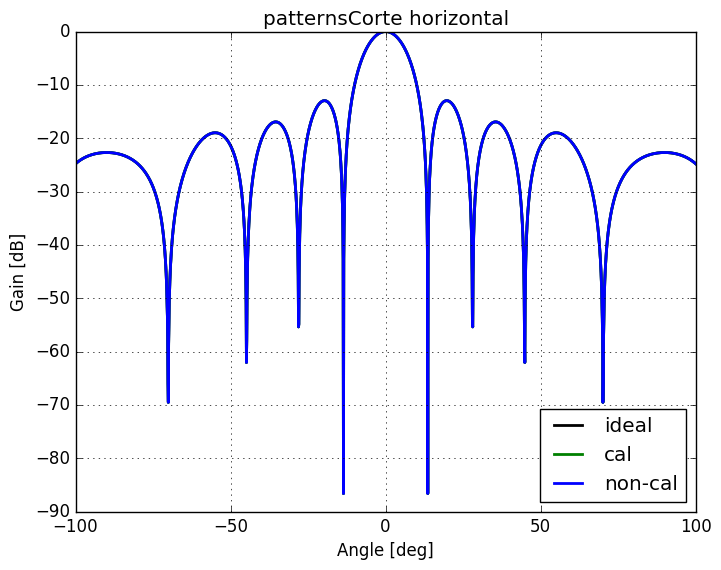
\includegraphics[width=7cm]{gfx/nonErrClassical10degRowAzCut.png}}
 	\subfloat[]{
		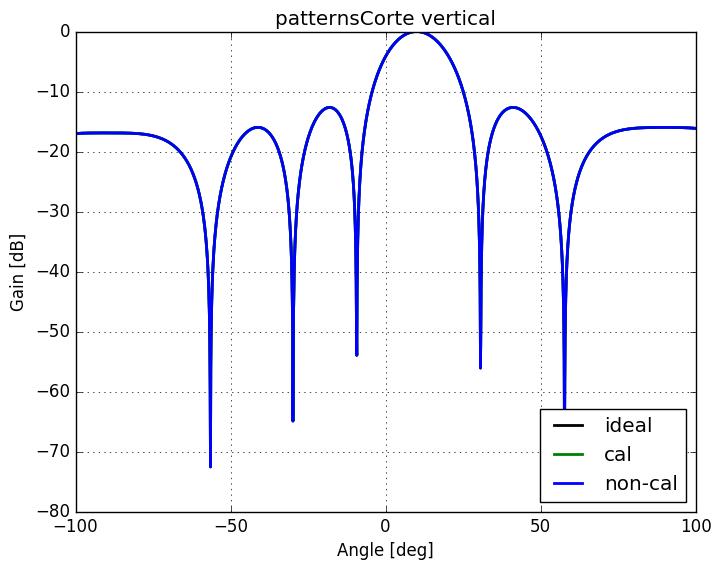
\includegraphics[width=7cm]{gfx/nonErrClassical10degRowElCut.png}}
	\caption{Correcciones de la señal transmitida utilizando calibración clásica. (a) ganancia y fase transmitida por módulos
		radiantes. (b) corte horizontal del diagrama transmitido y (c) corte vertical del diagrama transmitido.}
	\label{fig:nonErrClassical10degRow}
\end{figure}
\begin{table}[H]
  \footnotesize
  \centering
  \begin{tabular}{|c|c|p{2cm}|p{2.5cm}|p{2.5cm}|p{2.5cm}|}
    \cline{2-6}
    \multicolumn{1}{c|}{} & Corte & Ganancia - lóbulo izq. [dBc] & Ganancia - lóbulo central [dB] &
    Ganancia - lóbulo der. [dBc] & Ancho - lóbulo central -3dB \tabularnewline\hline
    \multirow{2}{2cm}{Pat. sin calibrar} & H & 12.97 & 39.34 & 12.97 & 12.0 \tabularnewline\cline{2-6}
     & V & 12.65 & 43.48 & 12.65 & 17.8 \tabularnewline\hline
    \multirow{2}{2cm}{Pat. calibrado} & H & 12.97 & 39.19 & 12.97 & 12.0 \tabularnewline\cline{2-6}
     & V & 12.65 & 43.34 & 12.65 & 17.8 \tabularnewline\hline
    \multirow{2}{2cm}{Pat. ideal} & H & 12.97 & 38.76 & 12.97 & 12.0 \tabularnewline\cline{2-6}
     & V & 12.65 & 42.9 & 12.65 & 17.8 \tabularnewline\hline
    \multirow{2}{2cm}{Dif. sin calibrar} & H & 0.0 & 0.58 & 0.0 & 0.0\tabularnewline\cline{2-6}
     & V & 0.0 & 0.58 & 0.0 & 0.0 \tabularnewline\hline
    \multirow{2}{2cm}{Dif. calibrado} & H & 0.0 & 0.43 & 0.0 & 0.0 \tabularnewline\cline{2-6}
     & V & 0.0 & 0.44 & 0.0 & 0.0 \tabularnewline\hline
  \end{tabular}
  \caption{Propiedades de los patrones calibrados y sin calibrar comparados con el ideal.}
  \label{tab:nonErrClassical10degRow}
\end{table}


\subsection{Utilizando la calibración con acoplamientos mútuos}


\subsubsection{Apuntamiento uniforme}

Los gráficos de la figura \ref{fig:nonErrMutual0deg} muestran que el calibrador funciona correctamente para estimar y corregir la 
fase y ganancia del sistema. Los diagramas de radiación calibrados resultan iguales al ideal.

En la tabla \ref{tab:nonErrMutual0deg} se puede apreciar como todos los parámetros de los diagramas calibrados resultan 
exactamente igual al ideal.

\begin{figure}[H]
	\centering
 	\subfloat[]{
		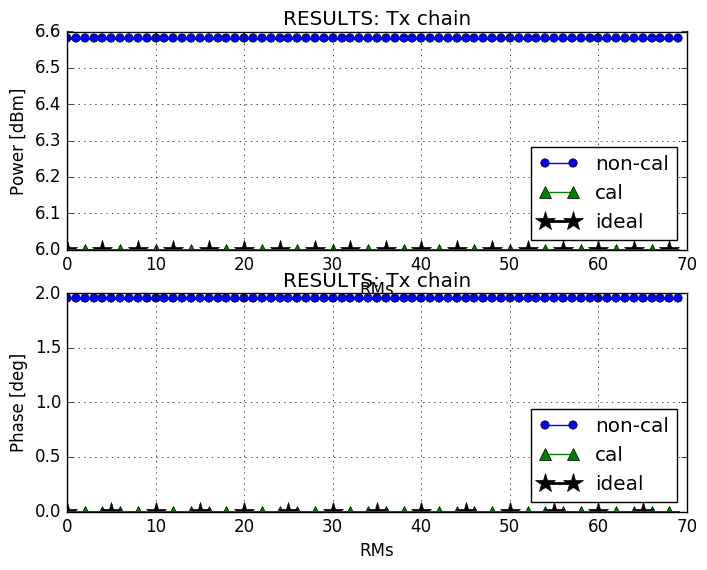
\includegraphics[width=9cm]{gfx/nonErrMutual0deg.png}}

	\subfloat[]{
		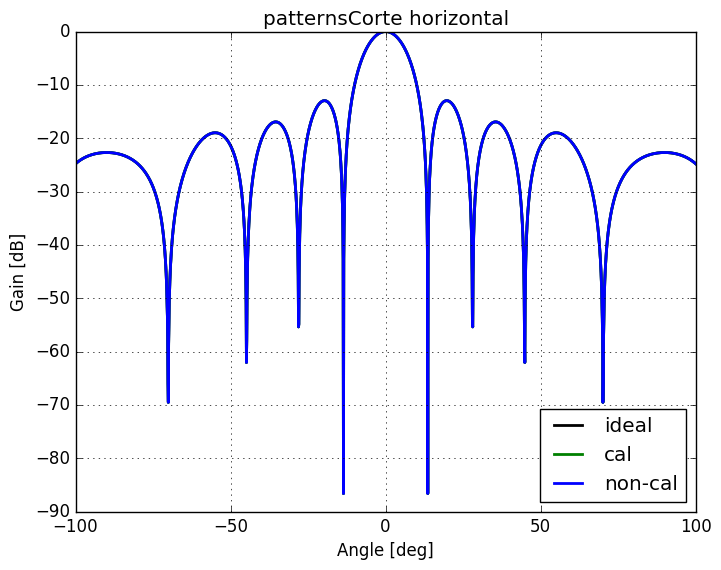
\includegraphics[width=7cm]{gfx/nonErrMutual0degAzCut.png}}
 	\subfloat[]{
		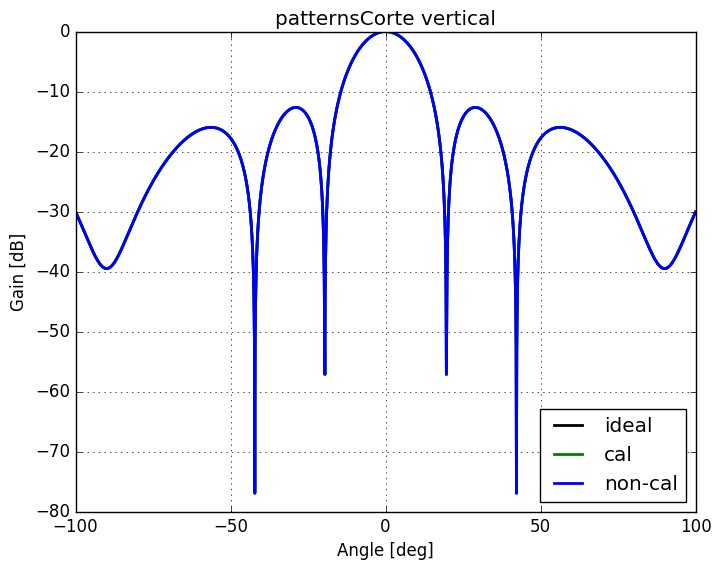
\includegraphics[width=7cm]{gfx/nonErrMutual0degElCut.png}}
	\caption{Correcciones de la señal transmitida utilizando calibración por acoplamientos mutuos. (a) ganancia y fase transmitida por módulos
		radiantes. (b) corte horizontal del diagrama transmitido y (c) corte vertical del diagrama transmitido.}
	\label{fig:nonErrMutual0deg}
\end{figure}

\begin{table}[H]
  \footnotesize
  \centering
  \begin{tabular}{|c|c|p{2cm}|p{2.5cm}|p{2.5cm}|p{2.5cm}|}
    \cline{2-6}
    \multicolumn{1}{c|}{} & Corte & Ganancia - lóbulo izq. [dBc] & Ganancia - lóbulo central [dB] &
    Ganancia - lóbulo der. [dBc] & Ancho - lóbulo central -3dB \tabularnewline\hline
    \multirow{2}{2cm}{Pat. sin calibrar} & H & 12.97 & 43.48 & 12.97 & 12.0 \tabularnewline\cline{2-6}
     & V & 12.65 & 43.48 & 12.65 & 17.4 \tabularnewline\hline
    \multirow{2}{2cm}{Pat. calibrado} & H & 12.97 & 42.9 & 12.97 & 12.0 \tabularnewline\cline{2-6}
     & V & 12.65 & 42.9 & 12.65 & 17.4 \tabularnewline\hline
    \multirow{2}{2cm}{Pat. ideal} & H & 12.97 & 42.9 & 12.97 & 12.0 \tabularnewline\cline{2-6}
     & V & 12.65 & 42.9 & 12.65 & 17.4 \tabularnewline\hline
    \multirow{2}{2cm}{Dif. sin calibrar} & H & 0.0 & 0.58 & 0.0 & 0.0\tabularnewline\cline{2-6}
     & V & 0.0 & 0.58 & 0.0 & 0.0 \tabularnewline\hline
    \multirow{2}{2cm}{Dif. calibrado} & H & 0.0 & 0.0 & 0.0 & 0.0 \tabularnewline\cline{2-6}
     & V & 0.0 & 0.0 & 0.0 & 0.0 \tabularnewline\hline
  \end{tabular}
  \caption{Propiedades de los patrones calibrados y sin calibrar comparados con el ideal.}
  \label{tab:nonErrMutual0deg}
\end{table}


\subsubsection{Apuntamiento 10 grados en dirección horizontal}

Los gráficos de la figura \ref{fig:nonErrMutual10degCol} muestran que el calibrador funciona correctamente para estimar y 
corregir la fase y ganancia del sistema utilizando un apuntamiento diferente al uniforme logrando así que los diagramas de 
radiación calibrados resultan iguales al ideal. A su vez, se puede apreciar que la fase muestra un diagrama estilo diente 
de sierra porque, al ser un apuntamiento horizontal, la fase entre columnas de la antena es diferente (y la numeración de 
los elementos radiantes es creciente de a filas).

En la tabla \ref{tab:nonErrMutual0deg} se puede apreciar como todos los parámetros de los diagramas calibrados resultan 
exactamente igual al ideal.

\begin{figure}[H]
	\centering
 	\subfloat[]{
		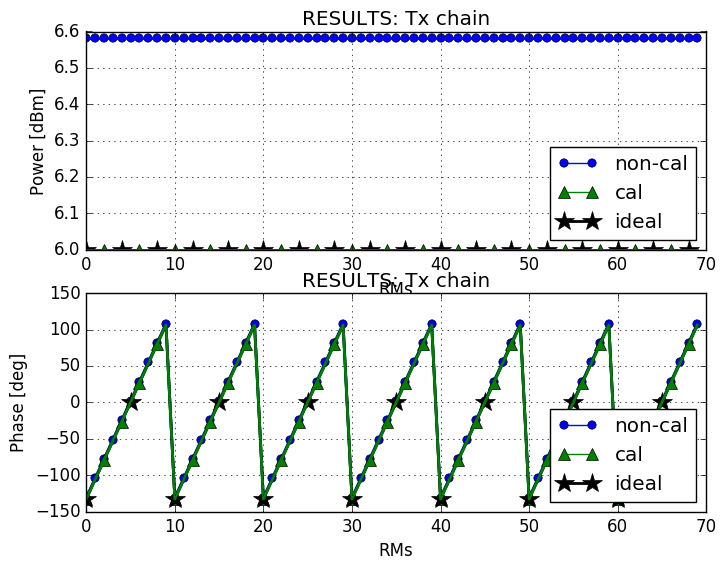
\includegraphics[width=9cm]{gfx/nonErrMutual10degCol.png}}

	\subfloat[]{
		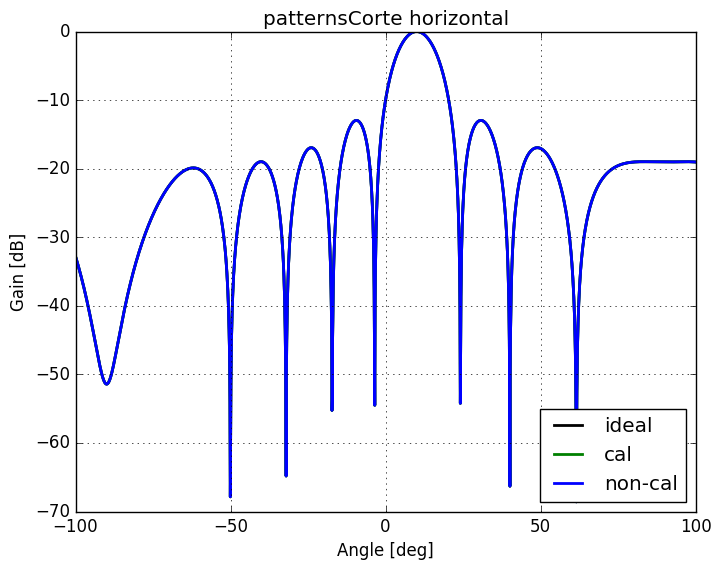
\includegraphics[width=7cm]{gfx/nonErrMutual10degColAzCut.png}}
 	\subfloat[]{
		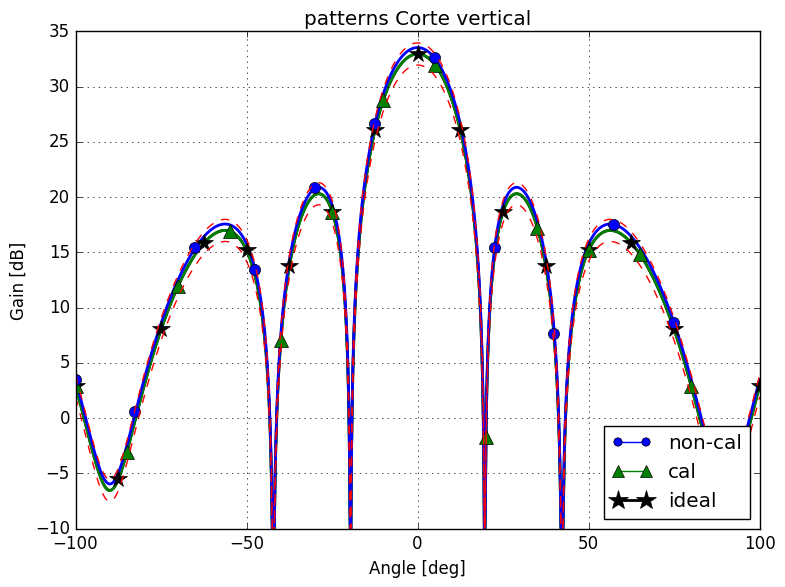
\includegraphics[width=7cm]{gfx/nonErrMutual10degColElCut.png}}
	\caption{Correcciones de la señal transmitida utilizando calibración por acoplamientos mutuos. (a) ganancia y fase 
		transmitida por módulos radiantes. (b) corte horizontal del diagrama transmitido y (c) corte vertical del diagrama transmitido.}
	\label{fig:nonErrMutual10degCol}
\end{figure}

\begin{table}[H]
  \footnotesize
  \centering
  \begin{tabular}{|c|c|p{2cm}|p{2.5cm}|p{2.5cm}|p{2.5cm}|}
    \cline{2-6}
    \multicolumn{1}{c|}{} & Corte & Ganancia - lóbulo izq. [dBc] & Ganancia - lóbulo central [dB] &
    Ganancia - lóbulo der. [dBc] & Ancho - lóbulo central -3dB \tabularnewline\hline
    \multirow{2}{2cm}{Pat. sin calibrar} & H & 12.97 & 43.48 & 12.97 & 12.4 \tabularnewline\cline{2-6}
     & V & 12.65 & 33.54 & 12.65 & 17.4 \tabularnewline\hline
    \multirow{2}{2cm}{Pat. calibrado} & H & 12.97 & 42.9 & 12.97 & 12.4 \tabularnewline\cline{2-6}
     & V & 12.65 & 32.96 & 12.65 & 17.4 \tabularnewline\hline
    \multirow{2}{2cm}{Pat. ideal} & H & 12.97 & 42.9 & 12.97 & 12.4 \tabularnewline\cline{2-6}
     & V & 12.65 & 32.96 & 12.65 & 17.4 \tabularnewline\hline
    \multirow{2}{2cm}{Dif. sin calibrar} & H & 0.0 & 0.58 & 0.0 & 0.0\tabularnewline\cline{2-6}
     & V & 0.0 & 0.58 & 0.0 & 0.0 \tabularnewline\hline
    \multirow{2}{2cm}{Dif. calibrado} & H & 0.0 & 0.0 & 0.0 & 0.0 \tabularnewline\cline{2-6}
     & V & 0.0 & 0.0 & 0.0 & 0.0 \tabularnewline\hline
  \end{tabular}
  \caption{Propiedades de los patrones calibrados y sin calibrar comparados con el ideal.}
  \label{tab:nonErrMutual10degCol}
\end{table}


\subsubsection{Apuntamiento 10 grados en dirección vertical}

Los gráficos de la figura \ref{fig:nonErrMutual10degRow} muestran que el calibrador funciona correctamente para estimar y 
corregir la fase y ganancia del sistema utilizando un apuntamiento diferente al uniforme logrando así que los diagramas de 
radiación calibrados resultan iguales al ideal. A su vez, se puede apreciar que la fase muestra un diagrama estilo escalonado
porque, al ser un apuntamiento vertical, la fase entre filas de la antena difiere (y la numeración de los elementos radiantes 
es creciente de a filas).

\begin{figure}[H]
	\centering
 	\subfloat[]{
		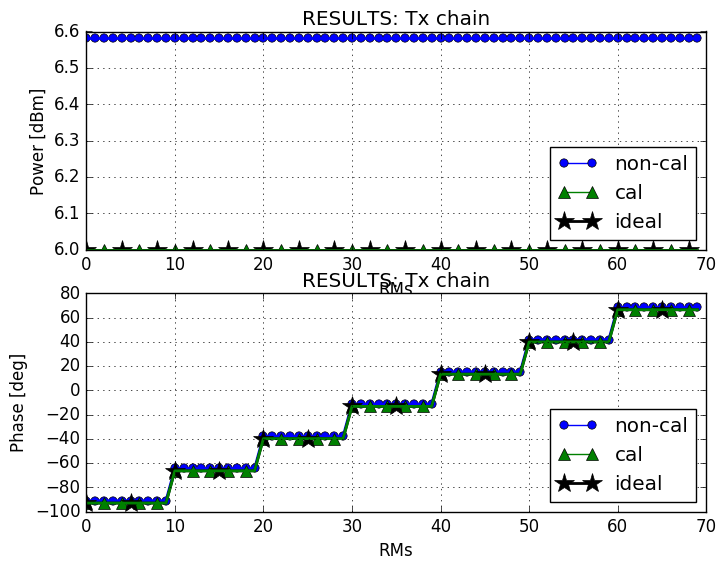
\includegraphics[width=9cm]{gfx/nonErrMutual10degRow.png}}

	\subfloat[]{
		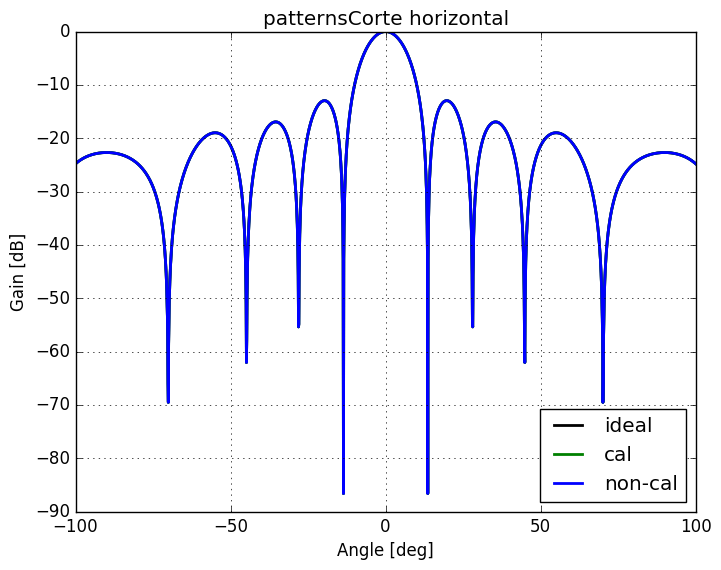
\includegraphics[width=7cm]{gfx/nonErrMutual10degRowAzCut.png}}
 	\subfloat[]{
		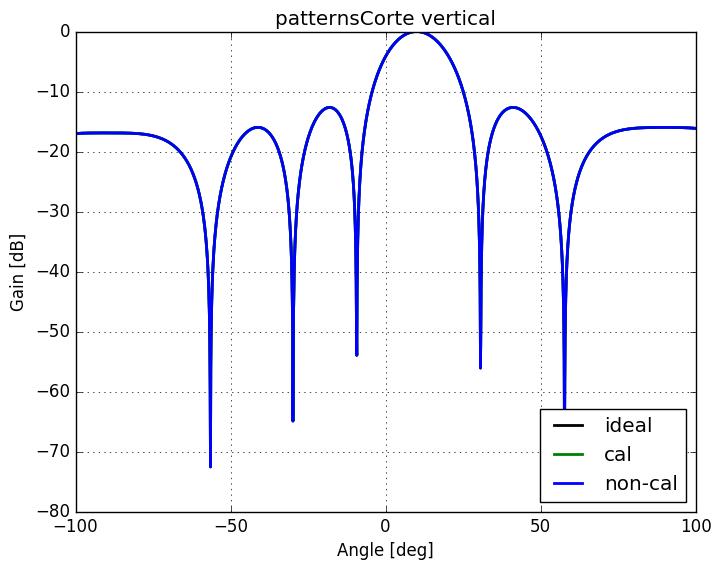
\includegraphics[width=7cm]{gfx/nonErrMutual10degRowElCut.png}}
	\caption{Correcciones de la señal transmitida utilizando calibración por acoplamientos mutuos. (a) ganancia y fase 
		transmitida por módulos radiantes. (b) corte horizontal del diagrama transmitido y (c) corte vertical del diagrama transmitido.}
	\label{fig:nonErrMutual10degRow}
\end{figure}

En la tabla \ref{tab:nonErrMutual10degRow} se puede apreciar como todos los parámetros de los diagramas calibrados resultan 
exactamente igual al ideal.

\begin{table}[H]
  \footnotesize
  \centering
  \begin{tabular}{|c|c|p{2cm}|p{2.5cm}|p{2.5cm}|p{2.5cm}|}
    \cline{2-6}
    \multicolumn{1}{c|}{} & Corte & Ganancia - lóbulo izq. [dBc] & Ganancia - lóbulo central [dB] &
    Ganancia - lóbulo der. [dBc] & Ancho - lóbulo central -3dB \tabularnewline\hline
    \multirow{2}{2cm}{Pat. sin calibrar} & H & 12.97 & 39.34 & 12.97 & 12.0 \tabularnewline\cline{2-6}
     & V & 12.65 & 43.48 & 12.65 & 17.8 \tabularnewline\hline
    \multirow{2}{2cm}{Pat. calibrado} & H & 12.97 & 38.76 & 12.97 & 12.0 \tabularnewline\cline{2-6}
     & V & 12.65 & 42.9 & 12.65 & 17.8 \tabularnewline\hline
    \multirow{2}{2cm}{Pat. ideal} & H & 12.97 & 38.76 & 12.97 & 12.0 \tabularnewline\cline{2-6}
     & V & 12.65 & 42.9 & 12.65 & 17.8 \tabularnewline\hline
    \multirow{2}{2cm}{Dif. sin calibrar} & H & 0.0 & 0.58 & 0.0 & 0.0\tabularnewline\cline{2-6}
     & V & 0.0 & 0.58 & 0.0 & 0.0 \tabularnewline\hline
    \multirow{2}{2cm}{Dif. calibrado} & H & 0.0 & 0.0 & 0.0 & 0.0 \tabularnewline\cline{2-6}
     & V & 0.0 & 0.0 & 0.0 & 0.0 \tabularnewline\hline
  \end{tabular}
  \caption{Propiedades de los patrones calibrados y sin calibrar comparados con el ideal.}
  \label{tab:nonErrMutual10degRow}
\end{table}


\section{Rotura de varios TRMs}
Los ensayos de esta sección tienen las siguientes caracterísiticas,
\begin{itemize}
	\item Salvo tres TRMs que están rotos, el resto de los componentes de antena no tienen ningún prolema de funcionamiento ni 
		desadaptaciones. Las posiciones de los TRMs son: [1,0], [3,4] y [5,5]. La nomenclatura de lectura es [fila, columna] con 
		valores desde 0.
	\item No hay errores de calibración.
	\item No hay errores en la señal.
\end{itemize}

\subsection{Utilizando la calibración clásica}
En las figuras \ref{fig:deadTRMsClassical0deg}, \ref{fig:deadTRMsClassical10degCol} y \ref{fig:deadTRMsClassical10degRow} se 
muestran los resultados de la calibración clásica para una antena con algunos TRMs destruidos. Se puede apreciar que no hay 
modificaciones en el comportamiento del método al calibrar el resto de los elementos y que el diagrama se deforma de una manera 
significativa.

\subsubsection{Apuntamiento uniforme}

Los gráficos de la figura \ref{fig:deadTRMsClassical0deg} muestran que el calibrador, dejando de lado la diferencia de 
estimación tanto de fase como ganancia por no abarcar la totalidad del sistema, funciona correctamente. Los elementos 10, 34 y 
55 presentan una ganancia que equivaldría al piso de ruido.

A causa de los TRMs muertos, se aprecia un aumento considerable de ambos lóbulos secundarios del corte horizontal. El corte 
vertical no presenta grandes desvíos.

\begin{figure}[H]
	\centering
 	\subfloat[]{
		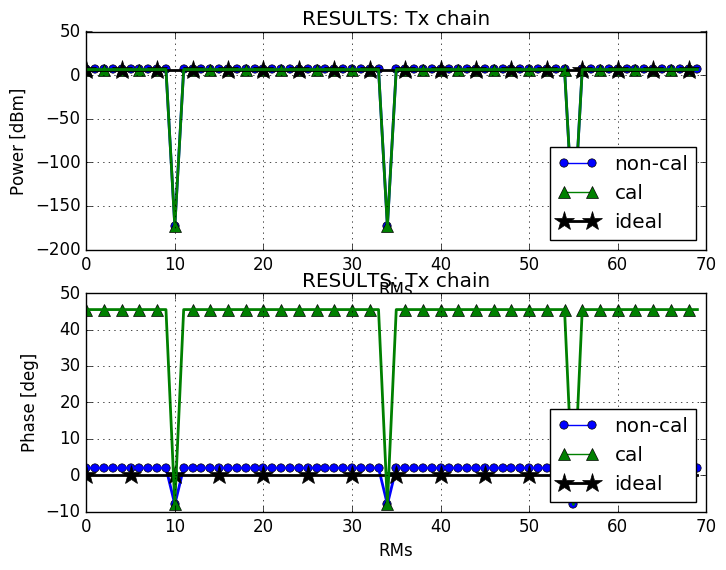
\includegraphics[width=9cm]{gfx/deadTRMsClassical0deg.png}}

	\subfloat[]{
		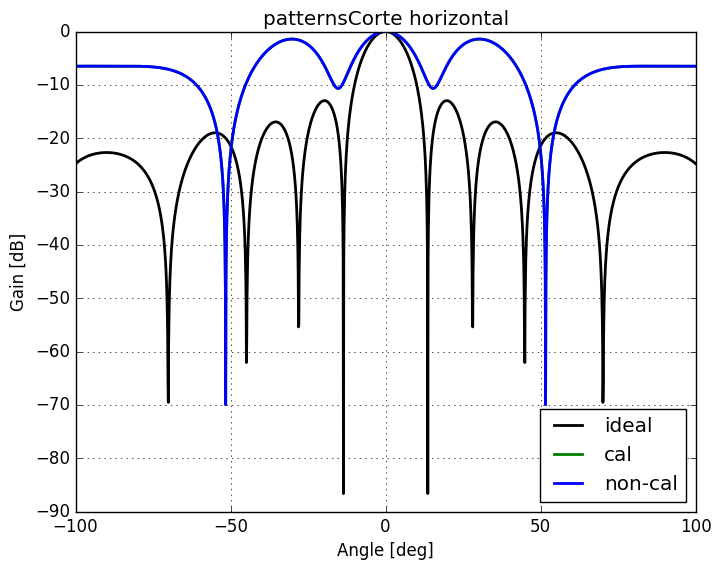
\includegraphics[width=7cm]{gfx/deadTRMsClassical0degAzCut.png}}
 	\subfloat[]{
		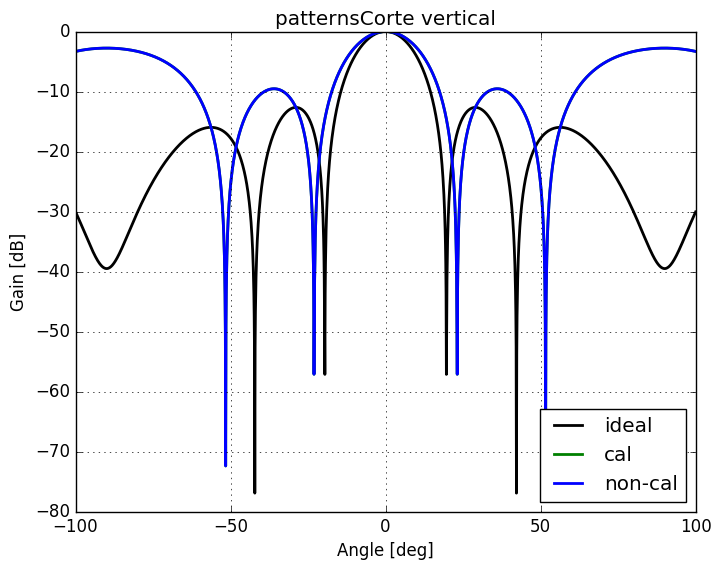
\includegraphics[width=7cm]{gfx/deadTRMsClassical0degElCut.png}}
	\caption{Correcciones de la señal transmitida utilizando calibración clásica. (a) ganancia y fase transmitida por módulos
		radiantes. (b) corte horizontal del diagrama transmitido y (c) corte vertical del diagrama transmitido.}
	\label{fig:deadTRMsClassical0deg}
\end{figure}

La tabla \ref{tab:deadTRMsClassical0deg} muestra que las diferencias de ganacia de los lóbulos secundarios entre los diagramas 
reales y el ideal para el corte horizontal ronda el dB y  este es el valor límite admisible. En el corte vertical esta 
diferencia es mucho menor.

\begin{table}[H]
  \footnotesize
  \centering
  \begin{tabular}{|c|c|p{2cm}|p{2.5cm}|p{2.5cm}|p{2.5cm}|}
    \cline{2-6}
    \multicolumn{1}{c|}{} & Corte & Ganancia - lóbulo izq. [dBc] & Ganancia - lóbulo central [dB] &
    Ganancia - lóbulo der. [dBc] & Ancho - lóbulo central -3dB \tabularnewline\hline
    \multirow{2}{2cm}{Pat. sin calibrar} & H & 11.93 & 43.1 & 11.93 & 12.0 \tabularnewline\cline{2-6}
     & V & 12.65 & 43.1 & 12.65 & 17.2 \tabularnewline\hline
    \multirow{2}{2cm}{Pat. calibrado} & H & 11.93 & 42.96 & 11.93 & 12.0 \tabularnewline\cline{2-6}
     & V & 12.65 & 42.96 & 12.65 & 17.2 \tabularnewline\hline
    \multirow{2}{2cm}{Pat. ideal} & H & 12.97 & 42.9 & 12.97 & 12.0 \tabularnewline\cline{2-6}
     & V & 12.65 & 42.9 & 12.65 & 17.4 \tabularnewline\hline
    \multirow{2}{2cm}{Dif. sin calibrar} & H & -1.04 & 0.2 & -1.04 & 0.0\tabularnewline\cline{2-6}
     & V & 0.0 & 0.2 & 0.0 & -0.2 \tabularnewline\hline
    \multirow{2}{2cm}{Dif. calibrado} & H & -1.04 & 0.06 & -1.04 & 0.0 \tabularnewline\cline{2-6}
     & V & 0.0 & 0.06 & 0.0 & -0.2 \tabularnewline\hline
  \end{tabular}
  \caption{Propiedades de los patrones calibrados y sin calibrar comparados con el ideal.}
  \label{tab:deadTRMsClassical0deg}
\end{table}


\subsubsection{Apuntamiento 10 grados en dirección horizontal}

Los gráficos de la figura \ref{fig:deadTRMsClassical10degCol} muestran que el calibrador, dejando de lado la diferencia de 
estimación tanto de fase como ganancia por no abarcar la totalidad del sistema, funciona correctamente. Los elementos 10, 34 y 
55 presentan una ganancia que equivaldría al piso de ruido.

A causa de los TRMs muertos, se aprecia un aumento considerable de ambos lóbulos secundarios de los cortes horizontal y vertical.

La tabla \ref{tab:deadTRMsClassical10degCol} muestra que las diferencias de ganacia de los lóbulos secundarios entre los 
diagramas de radiación reales y el ideal para el corte horizontal ronda el dB y para el vertical los dos dBs. Estas diferencias
ya son mayores a las permitidas por la máscara.

\begin{figure}[H]
	\centering
 	\subfloat[]{
		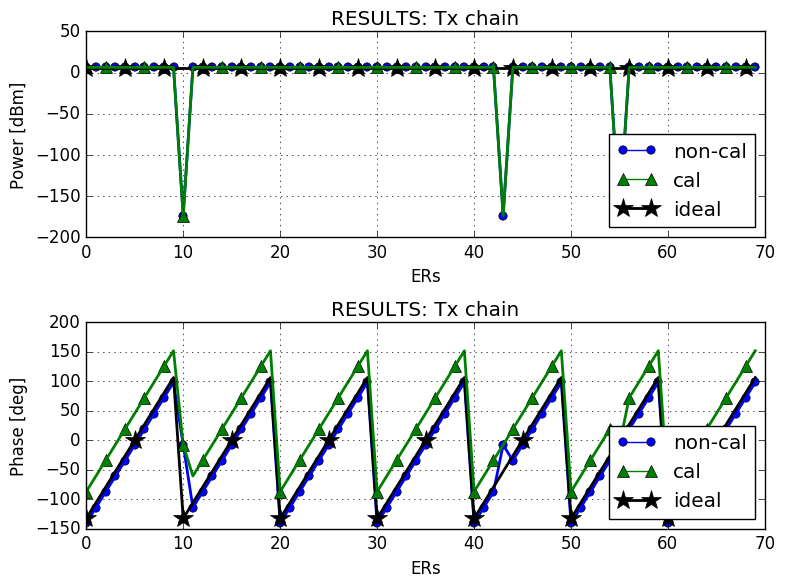
\includegraphics[width=9cm]{gfx/deadTRMsClassical10degCol.png}}

	\subfloat[]{
		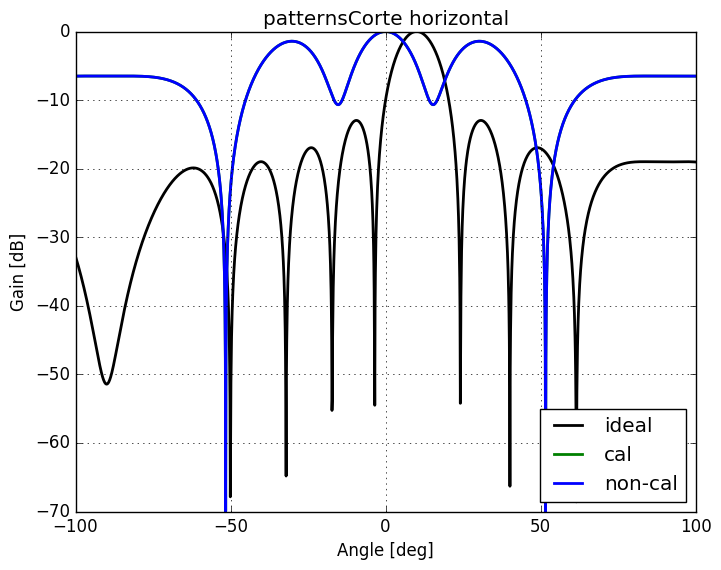
\includegraphics[width=7cm]{gfx/deadTRMsClassical10degColAzCut.png}}
 	\subfloat[]{
		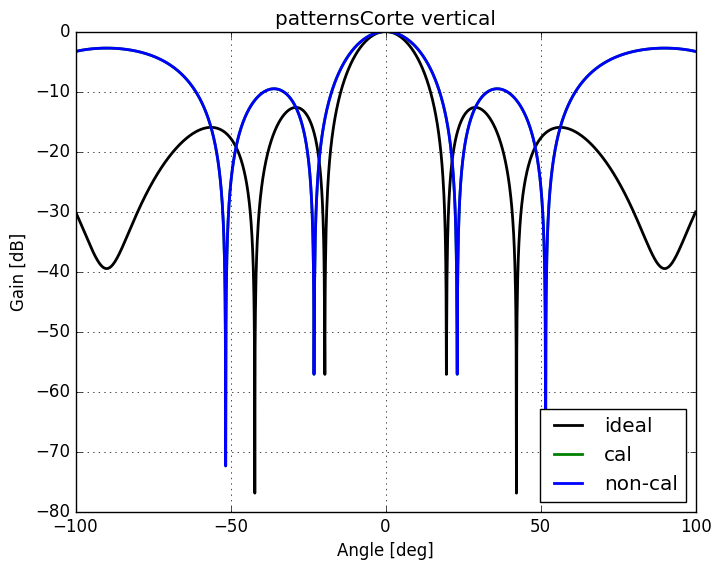
\includegraphics[width=7cm]{gfx/deadTRMsClassical10degColElCut.png}}
	\caption{Correcciones de la señal transmitida utilizando calibración clásica. (a) ganancia y fase transmitida por módulos
		radiantes. (b) corte horizontal del diagrama transmitido y (c) corte vertical del diagrama transmitido.}
	\label{fig:deadTRMsClassical10degCol}
\end{figure}
\begin{table}[H]
  \footnotesize
  \centering
  \begin{tabular}{|c|c|p{2cm}|p{2.5cm}|p{2.5cm}|p{2.5cm}|}
    \cline{2-6}
    \multicolumn{1}{c|}{} & Corte & Ganancia - lóbulo izq. [dBc] & Ganancia - lóbulo central [dB] &
    Ganancia - lóbulo der. [dBc] & Ancho - lóbulo central -3dB \tabularnewline\hline
    \multirow{2}{2cm}{Pat. sin calibrar} & H & 11.93 & 43.1 & 11.94 & 12.4 \tabularnewline\cline{2-6}
     & V & 11.91 & 32.98 & 10.26 & 16.8 \tabularnewline\hline
    \multirow{2}{2cm}{Pat. calibrado} & H & 11.93 & 42.96 & 11.94 & 12.4 \tabularnewline\cline{2-6}
     & V & 11.91 & 32.83 & 10.26 & 16.8 \tabularnewline\hline
    \multirow{2}{2cm}{Pat. ideal} & H & 12.97 & 42.9 & 12.97 & 12.4 \tabularnewline\cline{2-6}
     & V & 12.65 & 32.96 & 12.65 & 17.4 \tabularnewline\hline
    \multirow{2}{2cm}{Dif. sin calibrar} & H & -1.04 & 0.2 & -1.03 & 0.0\tabularnewline\cline{2-6}
     & V & -0.74 & 0.02 & -2.39 & -0.6 \tabularnewline\hline
    \multirow{2}{2cm}{Dif. calibrado} & H & -1.04 & 0.06 & -1.03 & 0.0 \tabularnewline\cline{2-6}
     & V & -0.74 & -0.13 & -2.39 & -0.6 \tabularnewline\hline
  \end{tabular}
  \caption{Propiedades de los patrones calibrados y sin calibrar comparados con el ideal.}
  \label{tab:deadTRMsClassical10degCol}
\end{table}


\subsubsection{Apuntamiento 10 grados en dirección vertical}

Los gráficos de la figura \ref{fig:deadTRMsClassical10degRow} muestran que el calibrador, dejando de lado la diferencia de 
estimación tanto de fase como ganancia por no abarcar la totalidad del sistema, funciona correctamente. Los elementos 10, 34 y 
55 presentan una ganancia que equivaldría al piso de ruido.

A causa de los TRMs muertos, se aprecia un aumento considerable de ambos lóbulos secundarios de los cortes horizontal y vertical.

\begin{figure}[H]
	\centering
 	\subfloat[]{
		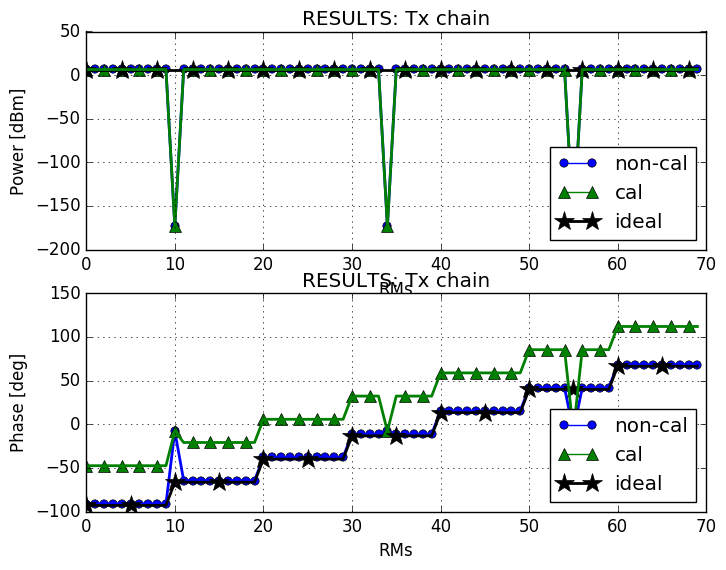
\includegraphics[width=9cm]{gfx/deadTRMsClassical10degRow.png}}

	\subfloat[]{
		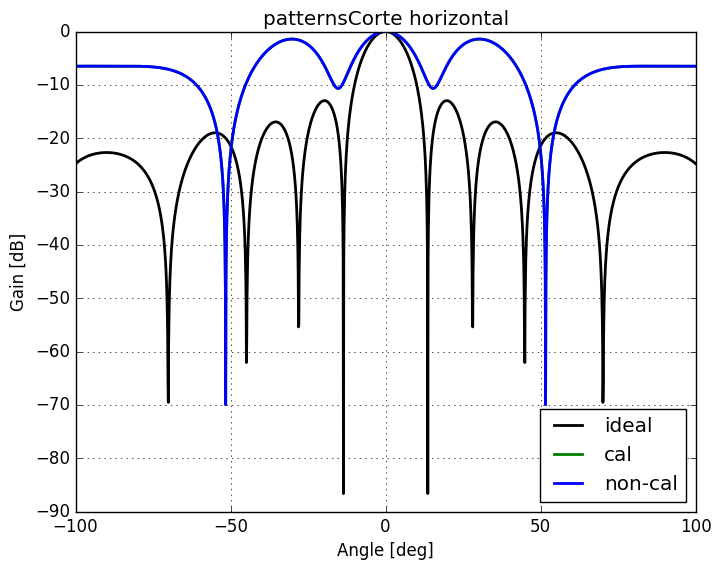
\includegraphics[width=7cm]{gfx/deadTRMsClassical10degRowAzCut.png}}
 	\subfloat[]{
		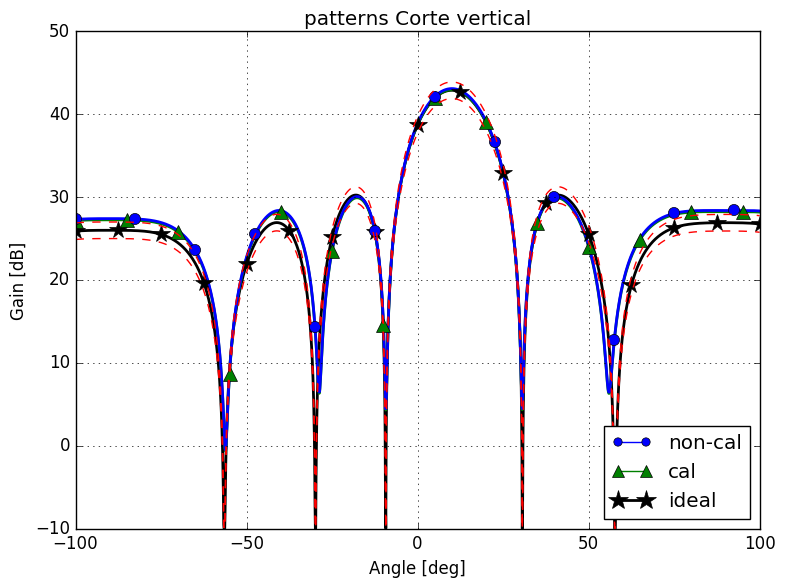
\includegraphics[width=7cm]{gfx/deadTRMsClassical10degRowElCut.png}}
	\caption{Correcciones de la señal transmitida utilizando calibración clásica. (a) ganancia y fase transmitida por módulos
		radiantes. (b) corte horizontal del diagrama transmitido y (c) corte vertical del diagrama transmitido.}
	\label{fig:deadTRMsClassical10degRow}
\end{figure}

La tabla \ref{tab:deadTRMsClassical10degRow} muestra que las diferencias de ganacia de los lóbulos secundarios entre los 
diagramas de radiación reales y el ideal para el corte horizontal supera el dB y para el vertical no se aprecian diferencias. 
Estas diferencias ya son mayores a las permitidas por la máscara.

\begin{table}[H]
  \footnotesize
  \centering
  \begin{tabular}{|c|c|p{2cm}|p{2.5cm}|p{2.5cm}|p{2.5cm}|}
    \cline{2-6}
    \multicolumn{1}{c|}{} & Corte & Ganancia - lóbulo izq. [dBc] & Ganancia - lóbulo central [dB] &
    Ganancia - lóbulo der. [dBc] & Ancho - lóbulo central -3dB \tabularnewline\hline
    \multirow{2}{2cm}{Pat. sin calibrar} & H & 11.29 & 38.89 & 11.81 & 12.0 \tabularnewline\cline{2-6}
     & V & 12.65 & 43.1 & 12.65 & 17.8 \tabularnewline\hline
    \multirow{2}{2cm}{Pat. calibrado} & H & 11.29 & 38.74 & 11.81 & 12.0 \tabularnewline\cline{2-6}
     & V & 12.65 & 42.96 & 12.65 & 17.8 \tabularnewline\hline
    \multirow{2}{2cm}{Pat. ideal} & H & 12.97 & 38.76 & 12.97 & 12.0 \tabularnewline\cline{2-6}
     & V & 12.65 & 42.9 & 12.65 & 17.8 \tabularnewline\hline
    \multirow{2}{2cm}{Dif. sin calibrar} & H & -1.68 & 0.13 & -1.16 & 0.0\tabularnewline\cline{2-6}
     & V & 0.0 & 0.2 & 0.0 & 0.0 \tabularnewline\hline
    \multirow{2}{2cm}{Dif. calibrado} & H & -1.68 & -0.02 & -1.16 & 0.0 \tabularnewline\cline{2-6}
     & V & 0.0 & 0.06 & 0.0 & 0.0 \tabularnewline\hline
  \end{tabular}
  \caption{Propiedades de los patrones calibrados y sin calibrar comparados con el ideal.}
  \label{tab:deadTRMsClassical10degRow}
\end{table}


\subsection{Utilizando la calibración con acoplamientos mútuos}

En las figuras \ref{fig:deadTRMsMutual0deg}, \ref{fig:deadTRMsMutual10degRow} y  \ref{fig:deadTRMsMutual10degCol} se puede 
observar que independientemente de que se hayan destruído varios TRMs, el método puede calibrar los lazos, obteniendo los 
valores deseados, tanto de fase como de ganancia del resto de los elementos.

\subsubsection{Apuntamiento uniforme}

Los gráficos de la figura \ref{fig:deadTRMsMutual0deg} muestran que el calibrador funciona correctamente. Los elementos 10, 
34 y 55 presentan una ganancia que equivaldría al piso de ruido.

A causa de los TRMs muertos, se aprecia un aumento considerable de ambos lóbulos secundarios del corte horizontal. El corte 
vertical no presenta un aumento en dicho parámetro pero sí un aumento en el ancho del lóbulo principal.

La tabla \ref{tab:deadTRMsMutual0deg} muestra que las diferencias de ganacia de los lóbulos secundarios entre los diagramas 
reales y el ideal para el corte horizontal ronda el dB y este es el valor límite admisible. En el corte vertical esta 
diferencia es nula, pero presenta 0.2 grados de incremento en el ancho del lóbulo principal. Se aprecia que la ganancia del 
lóbulo principal del diagrama de radiación calibrado es menor que la del ideal, esto se debe a la falta de energía que 
aportarían los elementos conectados a los TRMs que están muertos.

\begin{figure}[H]
	\centering
 	\subfloat[]{
		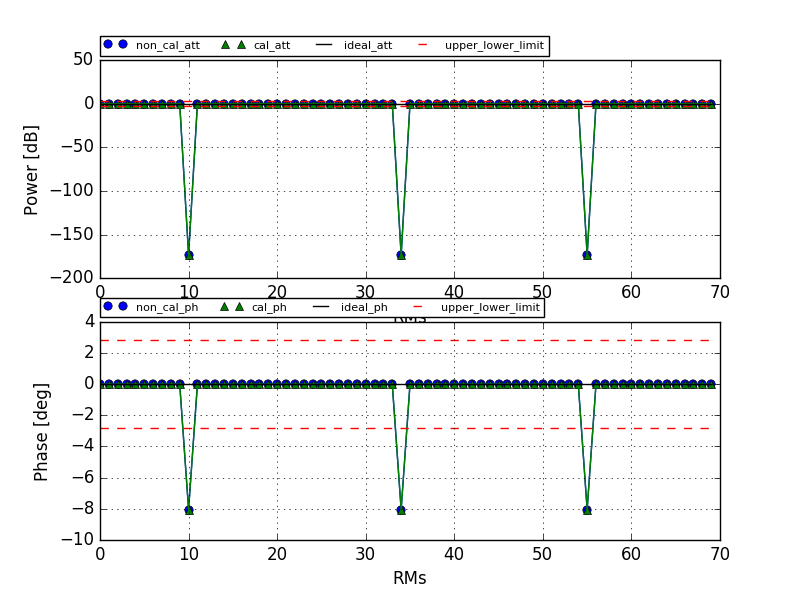
\includegraphics[width=9cm]{gfx/deadTRMsMutual0deg.png}}

	\subfloat[]{
		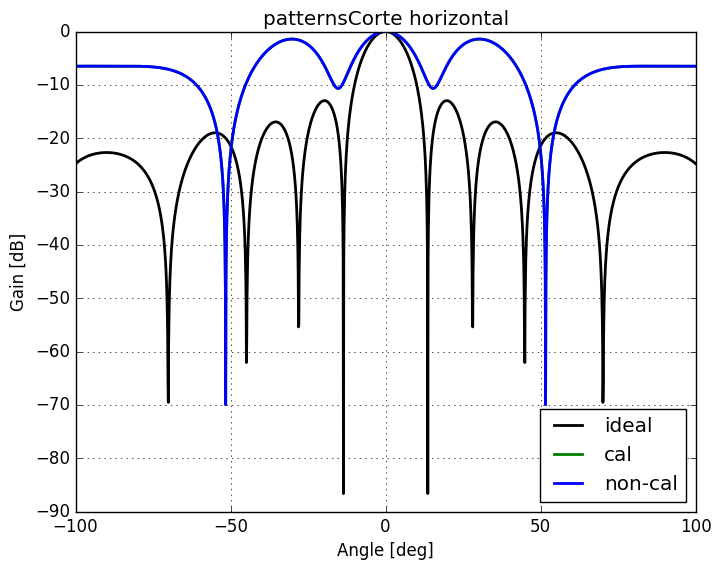
\includegraphics[width=7cm]{gfx/deadTRMsMutual0degAzCut.png}}
 	\subfloat[]{
		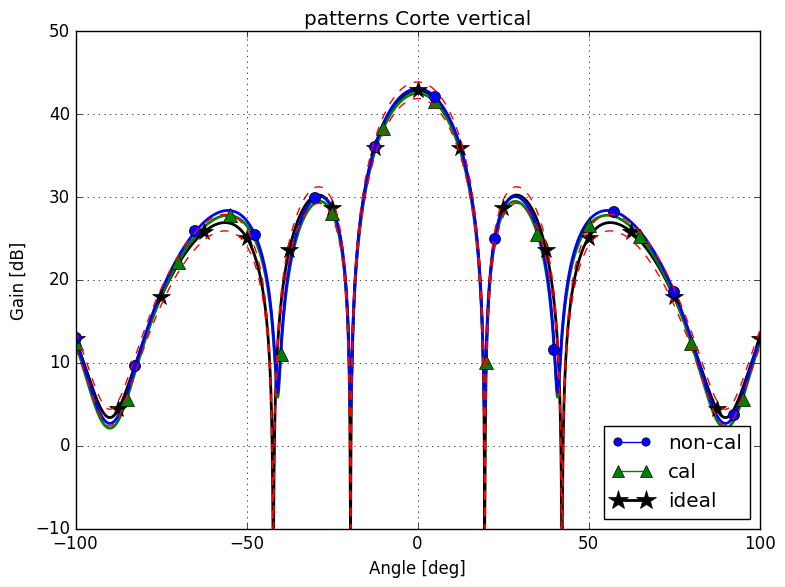
\includegraphics[width=7cm]{gfx/deadTRMsMutual0degElCut.png}}
	\caption{Correcciones de la señal transmitida utilizando calibración por acoplamientos mutuos. (a) ganancia y fase transmitida por módulos
		radiantes. (b) corte horizontal del diagrama transmitido y (c) corte vertical del diagrama transmitido.}
	\label{fig:deadTRMsMutual0deg}
\end{figure}
\begin{table}[H]
  \footnotesize
  \centering
  \begin{tabular}{|c|c|p{2cm}|p{2.5cm}|p{2.5cm}|p{2.5cm}|}
    \cline{2-6}
    \multicolumn{1}{c|}{} & Corte & Ganancia - lóbulo izq. [dBc] & Ganancia - lóbulo central [dB] &
    Ganancia - lóbulo der. [dBc] & Ancho - lóbulo central -3dB \tabularnewline\hline
    \multirow{2}{2cm}{Pat. sin calibrar} & H & 11.93 & 43.1 & 11.93 & 12.0 \tabularnewline\cline{2-6}
     & V & 12.65 & 43.1 & 12.65 & 17.2 \tabularnewline\hline
    \multirow{2}{2cm}{Pat. calibrado} & H & 11.93 & 42.52 & 11.93 & 12.0 \tabularnewline\cline{2-6}
     & V & 12.65 & 42.52 & 12.65 & 17.2 \tabularnewline\hline
    \multirow{2}{2cm}{Pat. ideal} & H & 12.97 & 42.9 & 12.97 & 12.0 \tabularnewline\cline{2-6}
     & V & 12.65 & 42.9 & 12.65 & 17.4 \tabularnewline\hline
    \multirow{2}{2cm}{Dif. sin calibrar} & H & -1.04 & 0.2 & -1.04 & 0.0\tabularnewline\cline{2-6}
     & V & 0.0 & 0.2 & 0.0 & -0.2 \tabularnewline\hline
    \multirow{2}{2cm}{Dif. calibrado} & H & -1.04 & -0.38 & -1.04 & 0.0 \tabularnewline\cline{2-6}
     & V & 0.0 & -0.38 & 0.0 & -0.2 \tabularnewline\hline
  \end{tabular}
  \caption{Propiedades de los patrones calibrados y sin calibrar comparados con el ideal.}
  \label{tab:deadTRMsMutual0deg}
\end{table}


\subsubsection{Apuntamiento 10 grados en dirección horizontal}

Los gráficos de la figura \ref{fig:deadTRMsMutual10degCol} muestran que el calibrador funciona correctamente. Los elementos 10, 
34 y 55 presentan una ganancia que equivaldría al piso de ruido.

A causa de los TRMs muertos, se aprecia un aumento considerable de ambos lóbulos secundarios del corte horizontal y vertical, 
a su vez un aumento en el ancho del lóbulo principal.

\begin{figure}[H]
	\centering
 	\subfloat[]{
		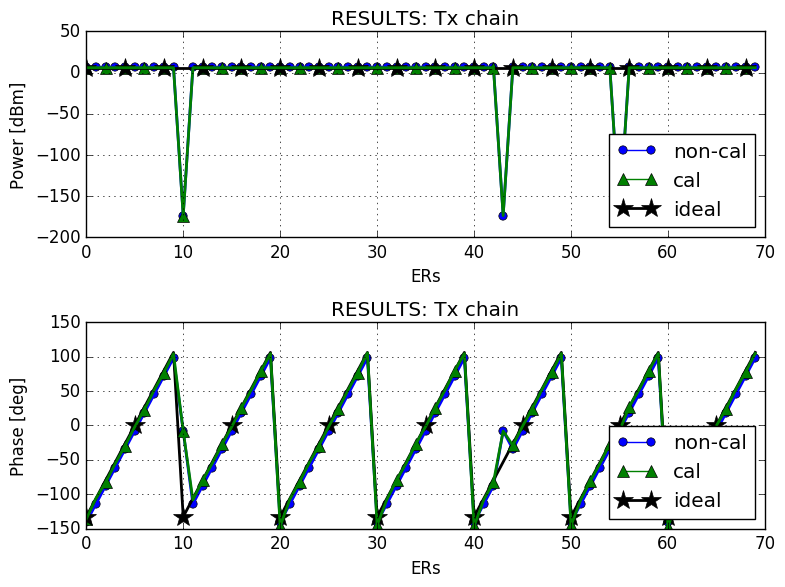
\includegraphics[width=9cm]{gfx/deadTRMsMutual10degCol.png}}

	\subfloat[]{
		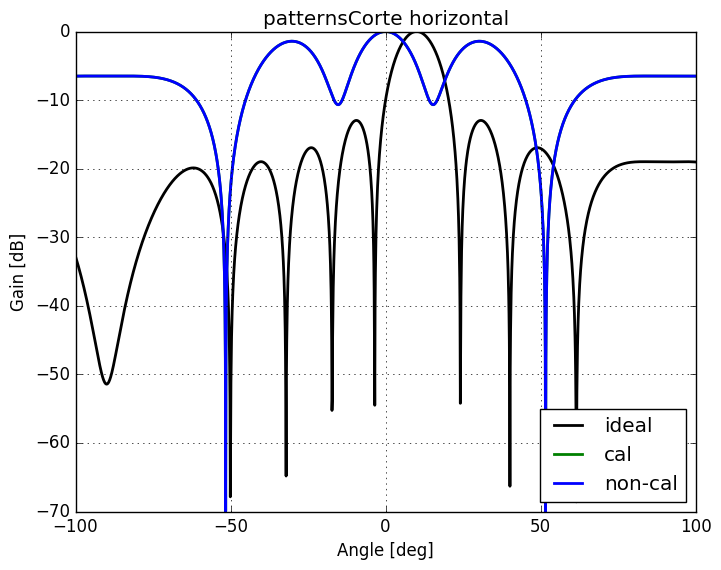
\includegraphics[width=7cm]{gfx/deadTRMsMutual10degColAzCut.png}}
 	\subfloat[]{
		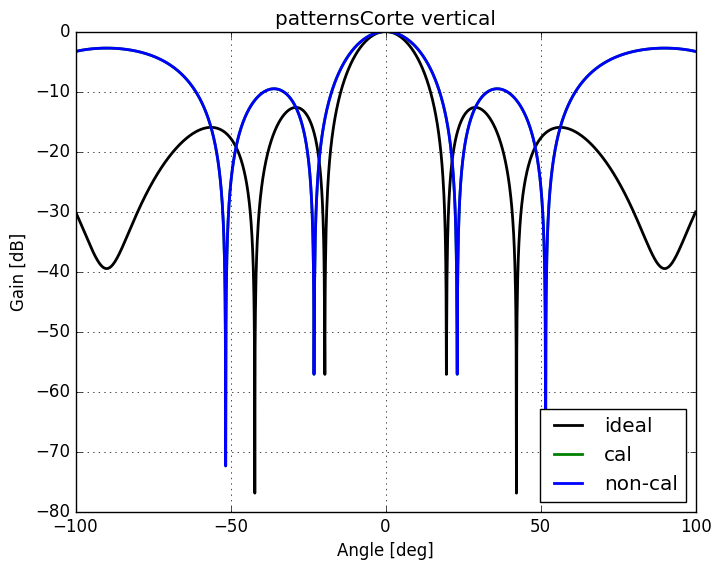
\includegraphics[width=7cm]{gfx/deadTRMsMutual10degColElCut.png}}
	\caption{Correcciones de la señal transmitida utilizando calibración por acoplamientos mutuos. (a) ganancia y fase 
		transmitida por módulos radiantes. (b) corte horizontal del diagrama transmitido y (c) corte vertical del diagrama transmitido.}
	\label{fig:deadTRMsMutual10degCol}
\end{figure}

La tabla \ref{tab:deadTRMsMutual10degCol} muestra que las diferencias de ganacia de los lóbulos secundarios entre los diagramas 
reales y el ideal para el corte horizontal ronda el dB y para el vertical los dos dBs. A su vez, el incremento del ancho del 
lóbulo principal es de 0.2 a 0.4 grados. La diferencia en ganancia del lóbulo principal del diagrama de radiación calibrado 
con respecto al ideal se debe a la falta de energía que aportarían los elementos conectados a los TRMs que están muertos.

\begin{table}[H]
  \footnotesize
  \centering
  \begin{tabular}{|c|c|p{2cm}|p{2.5cm}|p{2.5cm}|p{2.5cm}|}
    \cline{2-6}
    \multicolumn{1}{c|}{} & Corte & Ganancia - lóbulo izq. [dBc] & Ganancia - lóbulo central [dB] &
    Ganancia - lóbulo der. [dBc] & Ancho - lóbulo central -3dB \tabularnewline\hline
    \multirow{2}{2cm}{Pat. sin calibrar} & H & 11.93 & 43.1 & 11.94 & 12.4 \tabularnewline\cline{2-6}
     & V & 11.91 & 32.98 & 10.26 & 16.8 \tabularnewline\hline
    \multirow{2}{2cm}{Pat. calibrado} & H & 12.4 & 42.51 & 11.52 & 12.2 \tabularnewline\cline{2-6}
     & V & 11.63 & 32.04 & 9.96 & 17.0 \tabularnewline\hline
    \multirow{2}{2cm}{Pat. ideal} & H & 12.97 & 42.9 & 12.97 & 12.4 \tabularnewline\cline{2-6}
     & V & 12.65 & 32.96 & 12.65 & 17.4 \tabularnewline\hline
    \multirow{2}{2cm}{Dif. sin calibrar} & H & -1.04 & 0.2 & -1.03 & 0.0\tabularnewline\cline{2-6}
     & V & -0.74 & 0.02 & -2.39 & -0.6 \tabularnewline\hline
    \multirow{2}{2cm}{Dif. calibrado} & H & -0.57 & -0.39 & -1.45 & -0.2 \tabularnewline\cline{2-6}
     & V & -1.02 & -0.92 & -2.69 & -0.4 \tabularnewline\hline
  \end{tabular}
  \caption{Propiedades de los patrones calibrados y sin calibrar comparados con el ideal.}
  \label{tab:deadTRMsMutual10degCol}
\end{table}


\subsubsection{Apuntamiento 10 grados en dirección vertical}

En la figuras \ref{fig:nonErrMutual10degRow} se puede verificar que el apuntamiento es el correcto por los defasajes observados, 
como hay 10 elementos radiantes por fila, al apuntar verticalmente, cada fila posee un defasaje diferente, es por esta razón que 
la tercer fila se ve un gráfico estilo una escalera con siete escalones (que es la cantidad de columnas de la antena). A su vez, 
se aprecia que el calibrador lleva tanto la potencia como la fase transmitida al valor deseado.

La tabla \ref{tab:deadTRMsMutual10degRow} muestra que las diferencias de ganacia de los lóbulos secundarios entre los diagramas 
reales y el ideal para el corte horizontal ronda el dB y medio. El corte vertical no presenta incremento. La diferencia en 
ganancia del lóbulo principal del diagrama de radiación calibrado con respecto al ideal se debe a la falta de energía que 
aportarían los elementos conectados a los TRMs que están muertos.

\begin{figure}[H]
	\centering
 	\subfloat[]{
		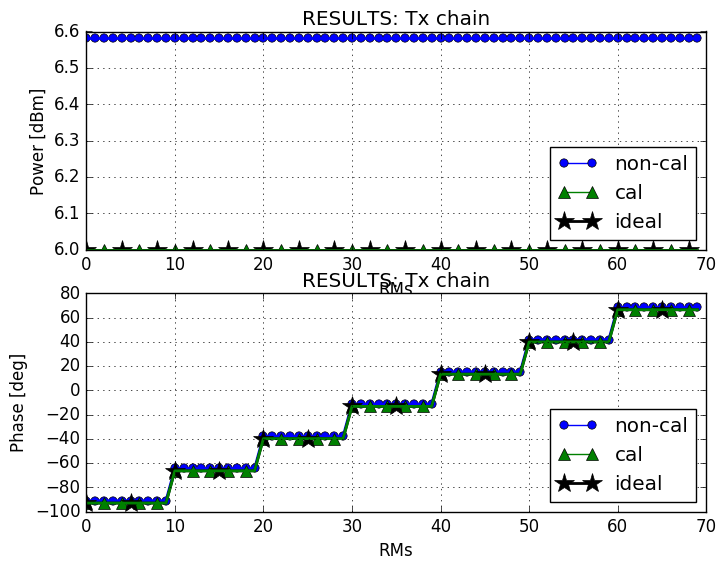
\includegraphics[width=9cm]{gfx/nonErrMutual10degRow.png}}

	\subfloat[]{
		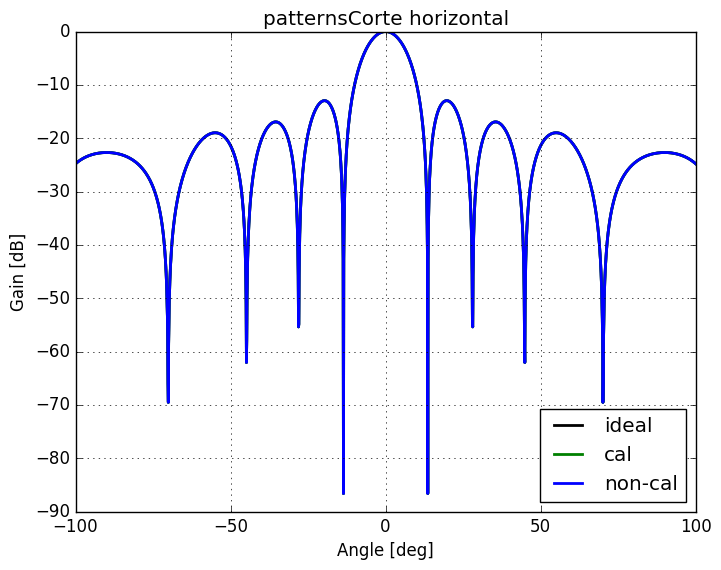
\includegraphics[width=7cm]{gfx/nonErrMutual10degRowAzCut.png}}
 	\subfloat[]{
		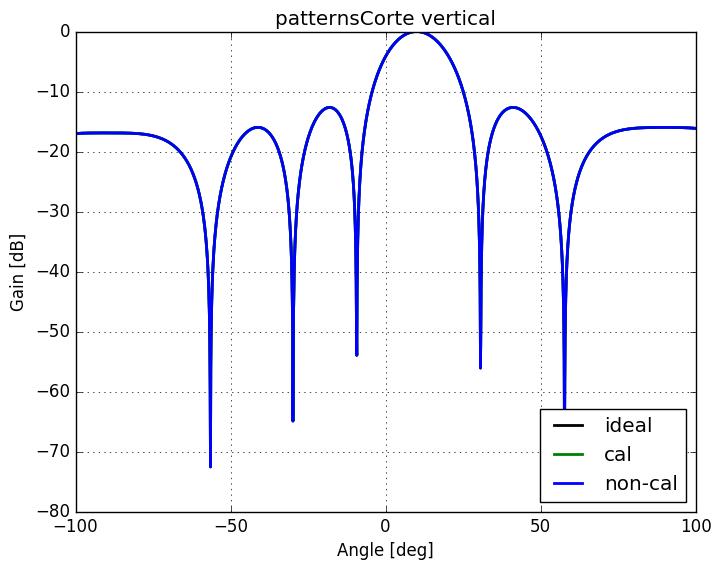
\includegraphics[width=7cm]{gfx/nonErrMutual10degRowElCut.png}}
	\caption{Correcciones de la señal transmitida utilizando calibración por acoplamientos mutuos. (a) ganancia y fase 
		transmitida por módulos radiantes. (b) corte horizontal del diagrama transmitido y (c) corte vertical del diagrama transmitido.}
	\label{fig:deadTRMsMutual10degRow}
\end{figure}

\begin{table}[H]
  \footnotesize
  \centering
  \begin{tabular}{|c|c|p{2cm}|p{2.5cm}|p{2.5cm}|p{2.5cm}|}
    \cline{2-6}
    \multicolumn{1}{c|}{} & Corte & Ganancia - lóbulo izq. [dBc] & Ganancia - lóbulo central [dB] &
    Ganancia - lóbulo der. [dBc] & Ancho - lóbulo central -3dB \tabularnewline\hline
    \multirow{2}{2cm}{Pat. sin calibrar} & H & 11.29 & 38.89 & 11.81 & 12.0 \tabularnewline\cline{2-6}
     & V & 12.65 & 43.1 & 12.65 & 17.8 \tabularnewline\hline
    \multirow{2}{2cm}{Pat. calibrado} & H & 11.29 & 38.31 & 11.81 & 12.0 \tabularnewline\cline{2-6}
     & V & 12.65 & 42.52 & 12.65 & 17.8 \tabularnewline\hline
    \multirow{2}{2cm}{Pat. ideal} & H & 12.97 & 38.76 & 12.97 & 12.0 \tabularnewline\cline{2-6}
     & V & 12.65 & 42.9 & 12.65 & 17.8 \tabularnewline\hline
    \multirow{2}{2cm}{Dif. sin calibrar} & H & -1.68 & 0.13 & -1.16 & 0.0\tabularnewline\cline{2-6}
     & V & 0.0 & 0.2 & 0.0 & 0.0 \tabularnewline\hline
    \multirow{2}{2cm}{Dif. calibrado} & H & -1.68 & -0.45 & -1.16 & 0.0 \tabularnewline\cline{2-6}
     & V & 0.0 & -0.38 & 0.0 & 0.0 \tabularnewline\hline
  \end{tabular}
  \caption{Propiedades de los patrones calibrados y sin calibrar comparados con el ideal.}
  \label{tab:deadTRMsMutual10degRow}
\end{table}


\section{Dispersiones en comportamiento de componentes de la antena}

Los ensayos de esta sección tienen las siguientes caracterísiticas,
\begin{itemize}
	\item Hay dispersiones de comportamiento en los siguientes componentes de la antena: circuladores, TRMs, PSCs y RMs. Las 
		magnitudes están especificadas en la tabla \ref{tab:errorReferences}.
		\begin{table}[H]
		  \footnotesize
		  \centering
		  \begin{tabular}{|c|c|}
			\hline
			\textbf{Dispersiones de componente} & \textbf{Desvío estandar} \tabularnewline \hline 
			Ganancia del circulador &  0.2 [dB] \tabularnewline\hline 
			Fase del circulador &  10 [deg] \tabularnewline\hline 
			Ganancia del TRM &  0.2 [dB] \tabularnewline\hline 
			Fase del TRM &  10 [deg] \tabularnewline\hline 
			Ganancia del PSC &  0.1 [dB] \tabularnewline\hline 
			Fase del PSC &  10 [deg] \tabularnewline\hline 
		  \end{tabular}
		  \caption{Configuración de los errores de componentes.}
		  \label{tab:errorReferences}
		\end{table}
	\item No hay errores de calibración.
	\item No hay errores en la señal.
\end{itemize}

\subsection{Utilizando la calibración clásica}

\subsubsection{Apuntamiento uniforme}

Los gráficos de la figura \ref{fig:compErrClassical0deg} muestran que el calibrador ya comienza a mostrar sus falencias no 
logrando calibrar la señal transmitida. En el corte vertical del diagrama de transmisión se aprecian más estas diferencias.

La tabla \ref{tab:compErrClassical0deg} muestra que las diferencias de ganacia de los lóbulos secundarios entre los diagramas 
reales y el ideal para el corte vertical supera el dB (valor límite admisible) y para el corte horizontal es de los 0.3 dB. No 
se aprecia una mejora en el ancho del lóbulo principal.
\begin{figure}[H]
	\centering
 	\subfloat[]{
		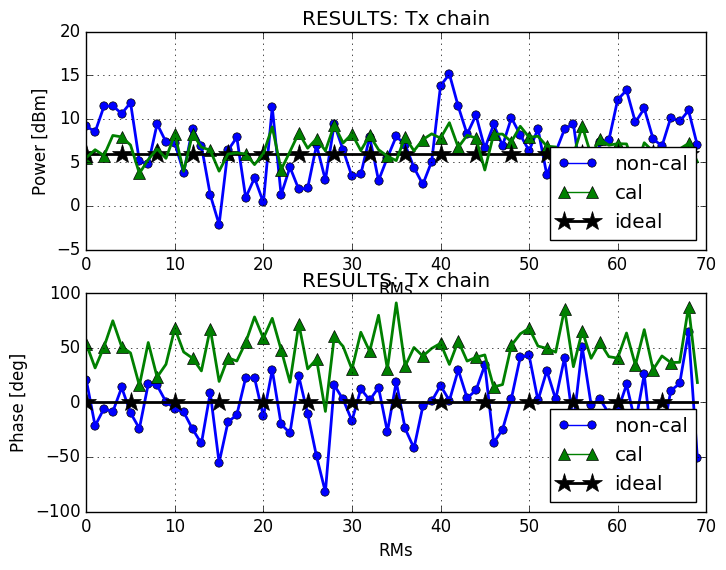
\includegraphics[width=9cm]{gfx/compErrClassical0deg.png}}

	\subfloat[]{
		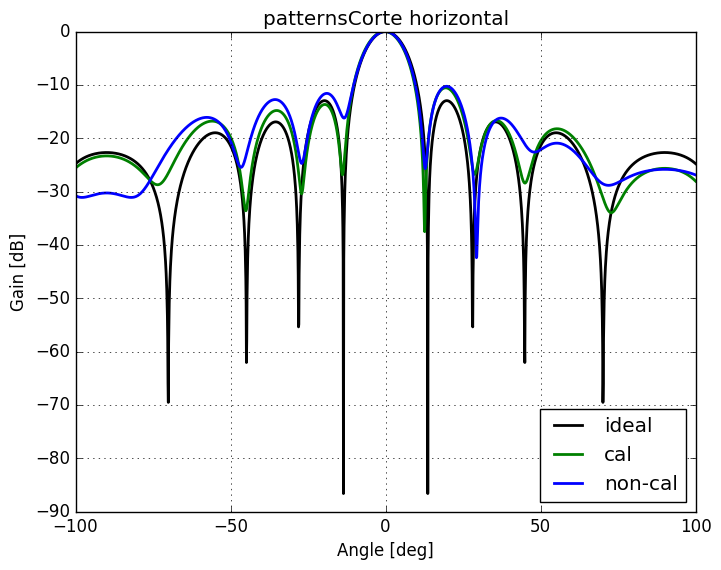
\includegraphics[width=7cm]{gfx/compErrClassical0degAzCut.png}}
 	\subfloat[]{
		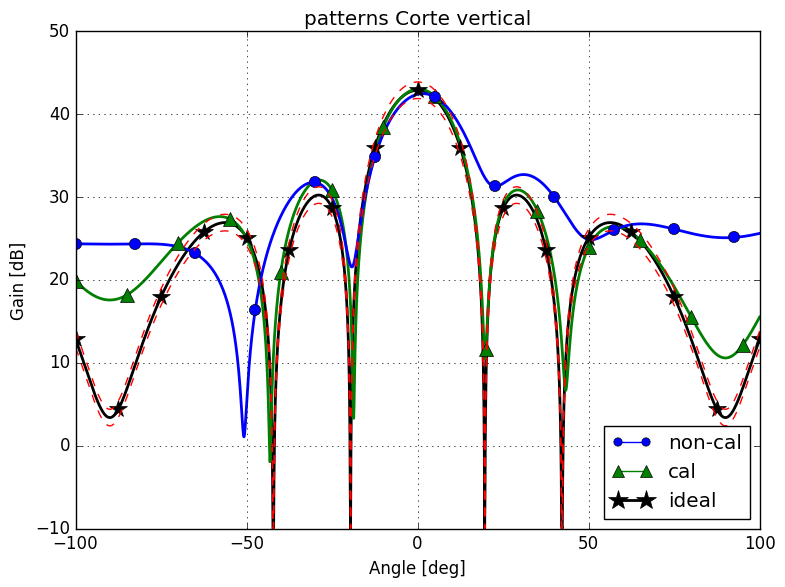
\includegraphics[width=7cm]{gfx/compErrClassical0degElCut.png}}
	\caption{Correcciones de la señal transmitida utilizando calibración clásica. (a) ganancia y fase transmitida por módulos
		radiantes. (b) corte horizontal del diagrama transmitido y (c) corte vertical del diagrama transmitido.}
	\label{fig:compErrClassical0deg}
\end{figure}
\begin{table}[H]
  \footnotesize
  \centering
  \begin{tabular}{|c|c|p{2cm}|p{2.5cm}|p{2.5cm}|p{2.5cm}|}
    \cline{2-6}
    \multicolumn{1}{c|}{} & Corte & Ganancia - lóbulo izq. [dBc] & Ganancia - lóbulo central [dB] &
    Ganancia - lóbulo der. [dBc] & Ancho - lóbulo central -3dB \tabularnewline\hline
    \multirow{2}{2cm}{Pat. sin calibrar} & H & 9.35 & 43.19 & 13.63 & 11.8 \tabularnewline\cline{2-6}
     & V & 11.12 & 43.19 & 10.93 & 16.2 \tabularnewline\hline
    \multirow{2}{2cm}{Pat. calibrado} & H & 13.25 & 43.26 & 14.49 & 12.4 \tabularnewline\cline{2-6}
     & V & 12.3 & 43.27 & 12.81 & 17.2 \tabularnewline\hline
    \multirow{2}{2cm}{Pat. ideal} & H & 12.97 & 42.9 & 12.97 & 12.0 \tabularnewline\cline{2-6}
     & V & 12.65 & 42.9 & 12.65 & 17.4 \tabularnewline\hline
    \multirow{2}{2cm}{Dif. sin calibrar} & H & -3.62 & 0.29 & 0.66 & -0.2\tabularnewline\cline{2-6}
     & V & -1.53 & 0.29 & -1.72 & -1.2 \tabularnewline\hline
    \multirow{2}{2cm}{Dif. calibrado} & H & 0.28 & 0.36 & 1.52 & 0.4 \tabularnewline\cline{2-6}
     & V & -0.35 & 0.37 & 0.16 & -0.2 \tabularnewline\hline
  \end{tabular}
  \caption{Propiedades de los patrones calibrados y sin calibrar comparados con el ideal.}
  \label{tab:compErrClassical0deg}
\end{table}


\subsubsection{Apuntamiento 10 grados en dirección horizontal}

En los gráficos de la figura \ref{fig:compErrClassical10degCol} se observa que el calibrador ya comienza a mostrar sus falencias no 
logrando calibrar completamente la señal transmitida. En el corte vertical del diagrama de transmisión se aprecian con mayor 
claridad estas diferencias.

La tabla \ref{tab:compErrClassical10degCol} muestra que las diferencias de ganacia de los lóbulos secundarios entre los diagramas 
reales y el ideal para ambos cortes supera el dB (valor límite admisible). A su vez se observa que el ancho del lóbulo 
principal se incrementa con la señal calibrada, logrando así una diferencia mayor con respecto al diagrama de radiación ideal.

\begin{figure}[H]
	\centering
 	\subfloat[]{
		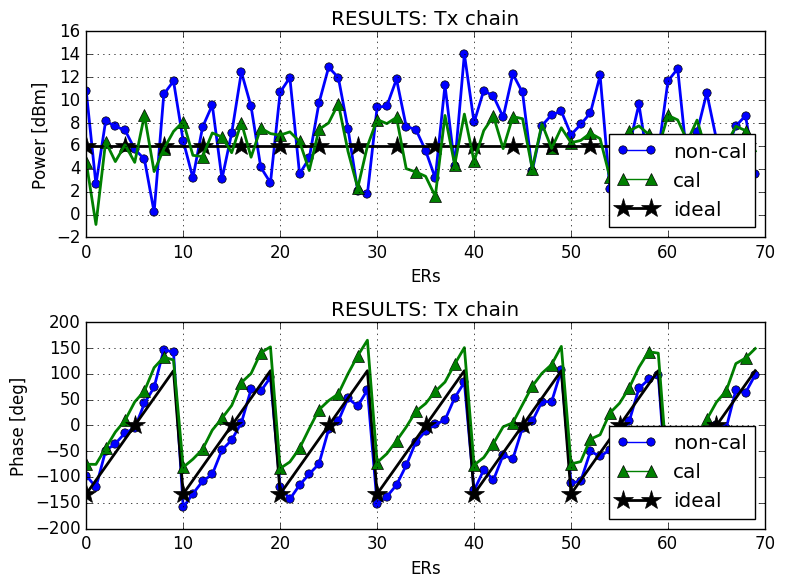
\includegraphics[width=9cm]{gfx/compErrClassical10degCol.png}}

	\subfloat[]{
		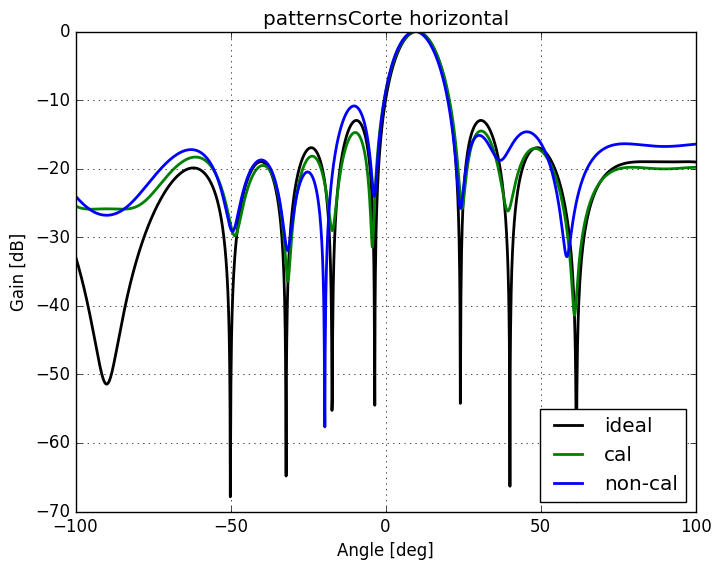
\includegraphics[width=7cm]{gfx/compErrClassical10degColAzCut.png}}
 	\subfloat[]{
		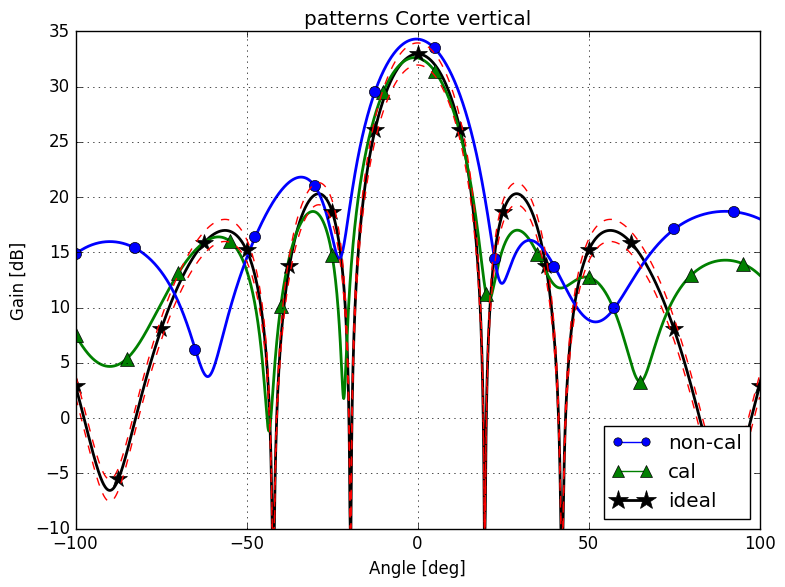
\includegraphics[width=7cm]{gfx/compErrClassical10degColElCut.png}}
	\caption{Correcciones de la señal transmitida utilizando calibración clásica. (a) ganancia y fase transmitida por módulos
		radiantes. (b) corte horizontal del diagrama transmitido y (c) corte vertical del diagrama transmitido.}
	\label{fig:compErrClassical10degCol}
\end{figure}

\begin{table}[H]
  \footnotesize
  \centering
  \begin{tabular}{|c|c|p{2cm}|p{2.5cm}|p{2.5cm}|p{2.5cm}|}
    \cline{2-6}
    \multicolumn{1}{c|}{} & Corte & Ganancia - lóbulo izq. [dBc] & Ganancia - lóbulo central [dB] &
    Ganancia - lóbulo der. [dBc] & Ancho - lóbulo central -3dB \tabularnewline\hline
    \multirow{2}{2cm}{Pat. sin calibrar} & H & 14.68 & 42.56 & 13.86 & 13.0 \tabularnewline\cline{2-6}
     & V & 7.37 & 34.13 & 11.18 & 16.4 \tabularnewline\hline
    \multirow{2}{2cm}{Pat. calibrado} & H & 13.7 & 42.97 & 14.44 & 12.8 \tabularnewline\cline{2-6}
     & V & 14.13 & 33.79 & 7.96 & 16.4 \tabularnewline\hline
    \multirow{2}{2cm}{Pat. ideal} & H & 12.97 & 42.9 & 12.97 & 12.4 \tabularnewline\cline{2-6}
     & V & 12.65 & 32.96 & 12.65 & 17.4 \tabularnewline\hline
    \multirow{2}{2cm}{Dif. sin calibrar} & H & 1.71 & -0.34 & 0.89 & 0.6\tabularnewline\cline{2-6}
     & V & -5.28 & 1.17 & -1.47 & -1.0 \tabularnewline\hline
    \multirow{2}{2cm}{Dif. calibrado} & H & 0.73 & 0.07 & 1.47 & 0.4 \tabularnewline\cline{2-6}
     & V & 1.48 & 0.83 & -4.69 & -1.0 \tabularnewline\hline
  \end{tabular}
  \caption{Propiedades de los patrones calibrados y sin calibrar comparados con el ideal.}
  \label{tab:compErrClassical10degCol}
\end{table}


\subsubsection{Apuntamiento 10 grados en dirección vertical}

En los gráficos de la figura \ref{fig:compErrClassical10degRow} se observa que el calibrador ya comienza a mostrar sus falencias no 
logrando calibrar completamente la señal transmitida. En el corte horizontal del diagrama de transmisión se aprecian con mayor 
claridad estas diferencias.

\begin{figure}[H]
	\centering
 	\subfloat[]{
		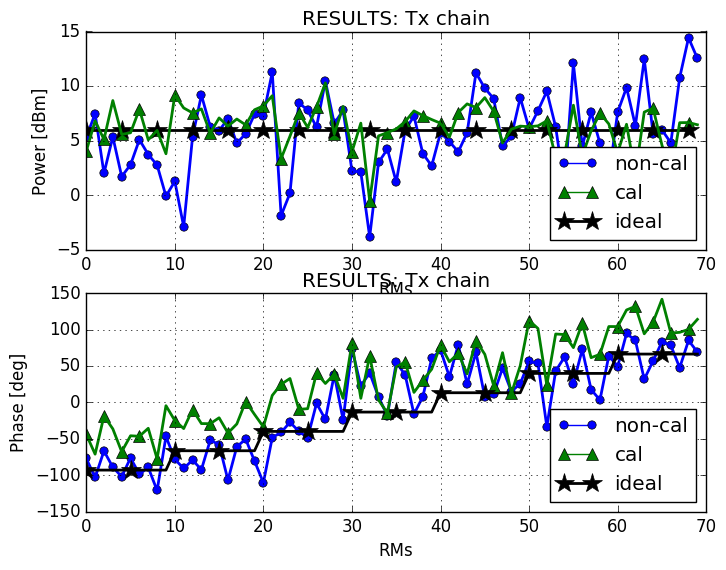
\includegraphics[width=9cm]{gfx/compErrClassical10degRow.png}}

	\subfloat[]{
		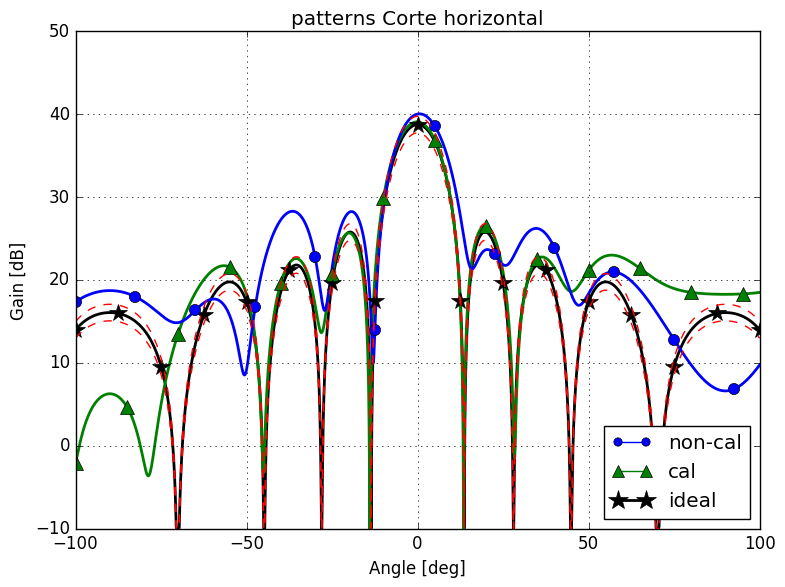
\includegraphics[width=7cm]{gfx/compErrClassical10degRowAzCut.png}}
 	\subfloat[]{
		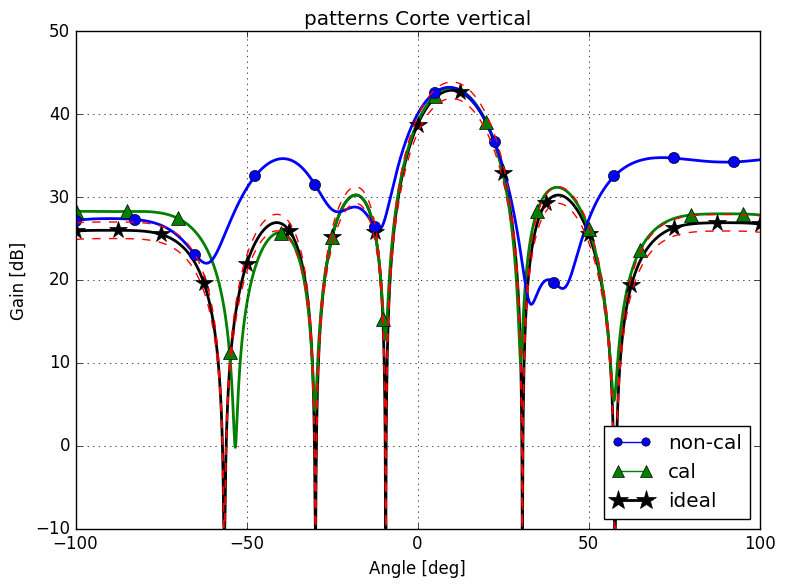
\includegraphics[width=7cm]{gfx/compErrClassical10degRowElCut.png}}
	\caption{Correcciones de la señal transmitida utilizando calibración clásica. (a) ganancia y fase transmitida por módulos
		radiantes. (b) corte horizontal del diagrama transmitido y (c) corte vertical del diagrama transmitido.}
	\label{fig:compErrClassical10degRow}
\end{figure}

La tabla \ref{tab:compErrClassical10degRow} muestra que las diferencias de ganacia de los lóbulos secundarios entre los diagramas 
reales y el ideal para ambos cortes supera el dB (valor límite admisible). A su vez se observa que el ancho del lóbulo 
principal se incrementa con la señal calibrada, logrando así una diferencia mayor con respecto al diagrama de radiación ideal.

\begin{table}[H]
  \footnotesize
  \centering
  \begin{tabular}{|c|c|p{2cm}|p{2.5cm}|p{2.5cm}|p{2.5cm}|}
    \cline{2-6}
    \multicolumn{1}{c|}{} & Corte & Ganancia - lóbulo izq. [dBc] & Ganancia - lóbulo central [dB] &
    Ganancia - lóbulo der. [dBc] & Ancho - lóbulo central -3dB \tabularnewline\hline
    \multirow{2}{2cm}{Pat. sin calibrar} & H & 10.36 & 39.16 & 18.48 & 13.0 \tabularnewline\cline{2-6}
     & V & 7.74 & 42.97 & 7.35 & 16.8 \tabularnewline\hline
    \multirow{2}{2cm}{Pat. calibrado} & H & 13.32 & 39.23 & 13.77 & 12.4 \tabularnewline\cline{2-6}
     & V & 12.09 & 43.25 & 11.74 & 17.6 \tabularnewline\hline
    \multirow{2}{2cm}{Pat. ideal} & H & 12.97 & 38.76 & 12.97 & 12.0 \tabularnewline\cline{2-6}
     & V & 12.65 & 42.9 & 12.65 & 17.8 \tabularnewline\hline
    \multirow{2}{2cm}{Dif. sin calibrar} & H & -2.61 & 0.4 & 5.51 & 1.0\tabularnewline\cline{2-6}
     & V & -4.91 & 0.07 & -5.3 & -1.0 \tabularnewline\hline
    \multirow{2}{2cm}{Dif. calibrado} & H & 0.35 & 0.47 & 0.8 & 0.4 \tabularnewline\cline{2-6}
     & V & -0.56 & 0.35 & -0.91 & -0.2 \tabularnewline\hline
  \end{tabular}
  \caption{Propiedades de los patrones calibrados y sin calibrar comparados con el ideal.}
  \label{tab:compErrClassical10degRow}
\end{table}


\subsection{Utilizando la calibración con acoplamientos mútuos}

\subsubsection{Apuntamiento uniforme}

Los gráficos de la figura \ref{fig:compErrMutual0deg} muestran que el calibrador funciona correctamente y que los diagramas de 
radiación de la señal calibrada se asemejan al ideal. 

La tabla \ref{tab:compErrMutual0deg} muestra que las diferencias de ganacia de los lóbulos secundarios entre los diagramas 
reales y el ideal para ambos cortes están dentro de la máscara admisible. A su vez, también se observa la mejora en el ancho 
del lóbulo principal. 

\begin{figure}[H]
	\centering
 	\subfloat[]{
		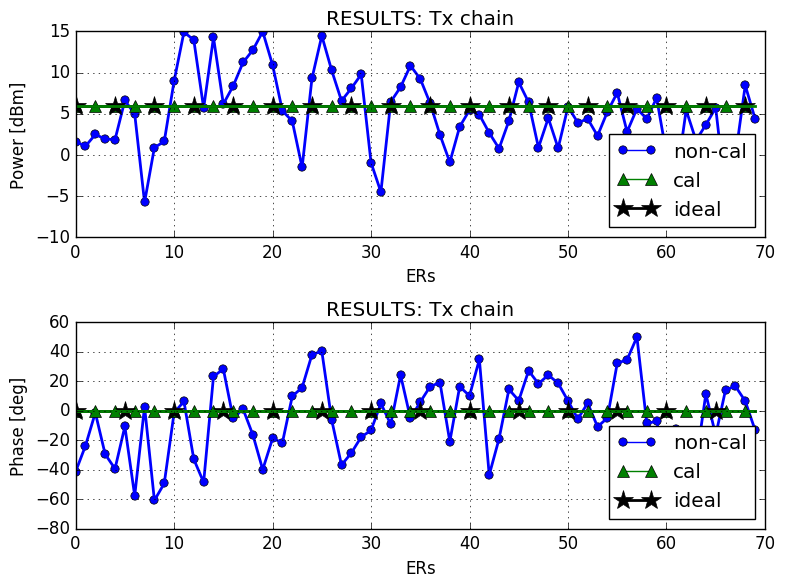
\includegraphics[width=9cm]{gfx/compErrMutual0deg.png}}

	\subfloat[]{
		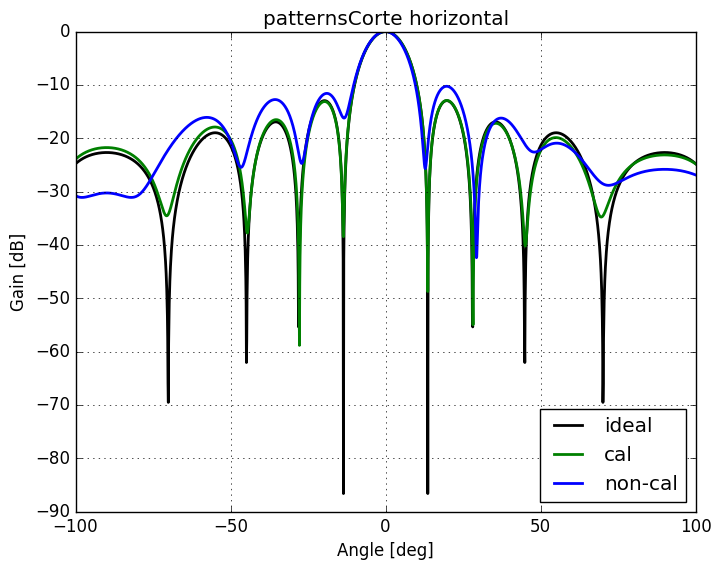
\includegraphics[width=7cm]{gfx/compErrMutual0degAzCut.png}}
 	\subfloat[]{
		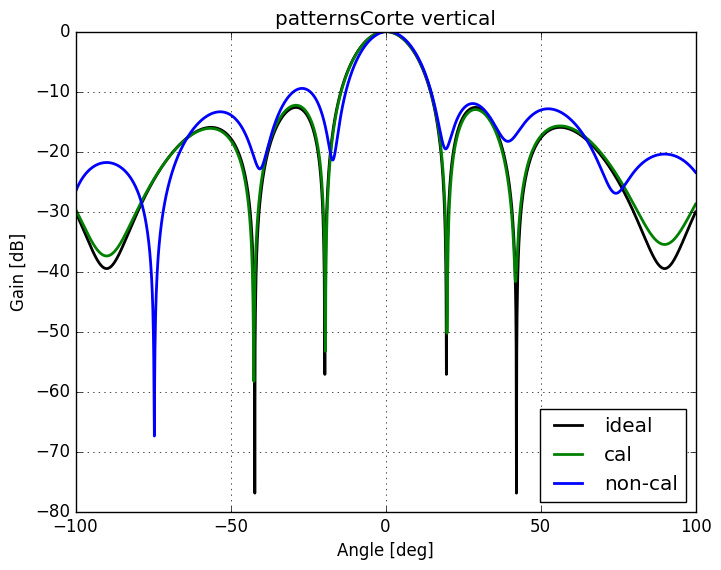
\includegraphics[width=7cm]{gfx/compErrMutual0degElCut.png}}
	\caption{Correcciones de la señal transmitida utilizando calibración por acoplamientos mutuos. (a) ganancia y fase transmitida por módulos
		radiantes. (b) corte horizontal del diagrama transmitido y (c) corte vertical del diagrama transmitido.}
	\label{fig:compErrMutual0deg}
\end{figure}

\begin{table}[H]
  \footnotesize
  \centering
  \begin{tabular}{|c|c|p{2cm}|p{2.5cm}|p{2.5cm}|p{2.5cm}|}
    \cline{2-6}
    \multicolumn{1}{c|}{} & Corte & Ganancia - lóbulo izq. [dBc] & Ganancia - lóbulo central [dB] &
    Ganancia - lóbulo der. [dBc] & Ancho - lóbulo central -3dB \tabularnewline\hline
    \multirow{2}{2cm}{Pat. sin calibrar} & H & 9.35 & 43.19 & 13.63 & 11.8 \tabularnewline\cline{2-6}
     & V & 11.12 & 43.19 & 10.93 & 16.2 \tabularnewline\hline
    \multirow{2}{2cm}{Pat. calibrado} & H & 12.97 & 42.9 & 12.97 & 12.0 \tabularnewline\cline{2-6}
     & V & 12.65 & 42.9 & 12.65 & 17.4 \tabularnewline\hline
    \multirow{2}{2cm}{Pat. ideal} & H & 12.97 & 42.9 & 12.97 & 12.0 \tabularnewline\cline{2-6}
     & V & 12.65 & 42.9 & 12.65 & 17.4 \tabularnewline\hline
    \multirow{2}{2cm}{Dif. sin calibrar} & H & -3.62 & 0.29 & 0.66 & -0.2\tabularnewline\cline{2-6}
     & V & -1.53 & 0.29 & -1.72 & -1.2 \tabularnewline\hline
    \multirow{2}{2cm}{Dif. calibrado} & H & 0.0 & 0.0 & 0.0 & 0.0 \tabularnewline\cline{2-6}
     & V & 0.0 & 0.0 & 0.0 & 0.0 \tabularnewline\hline
  \end{tabular}
  \caption{Propiedades de los patrones calibrados y sin calibrar comparados con el ideal.}
  \label{tab:compErrMutual0deg}
\end{table}


\subsubsection{Apuntamiento 10 grados en dirección horizontal}

Los gráficos de la figura \ref{fig:compErrMutual10degCol} muestran que el calibrador funciona correctamente y que los diagramas de 
radiación de la señal calibrada se asemejan al ideal. 

La tabla \ref{tab:compErrMutual10degCol} muestra que las diferencias de ganacia de los lóbulos secundarios entre los diagramas 
reales y el ideal para ambos cortes están dentro de la máscara admisible. A su vez, también se observa la mejora en el ancho 
del lóbulo principal.

\begin{figure}[H]
	\centering
 	\subfloat[]{
		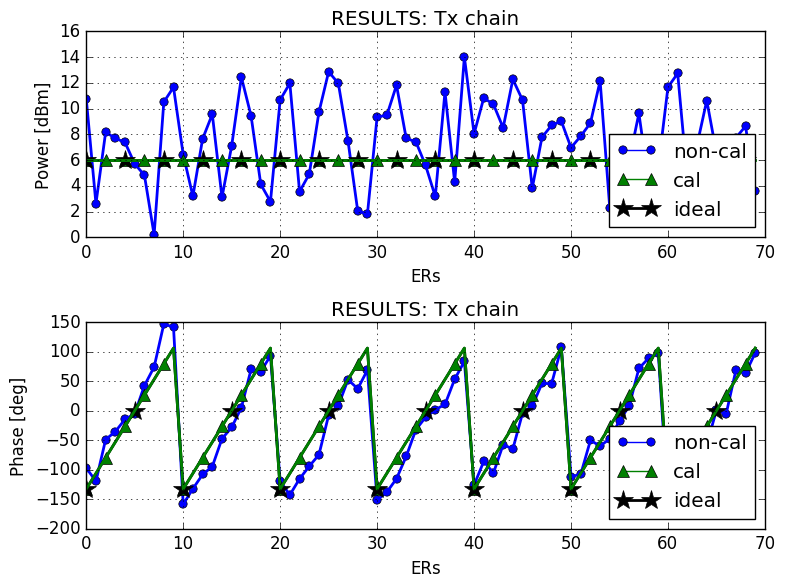
\includegraphics[width=9cm]{gfx/compErrMutual10degCol.png}}

	\subfloat[]{
		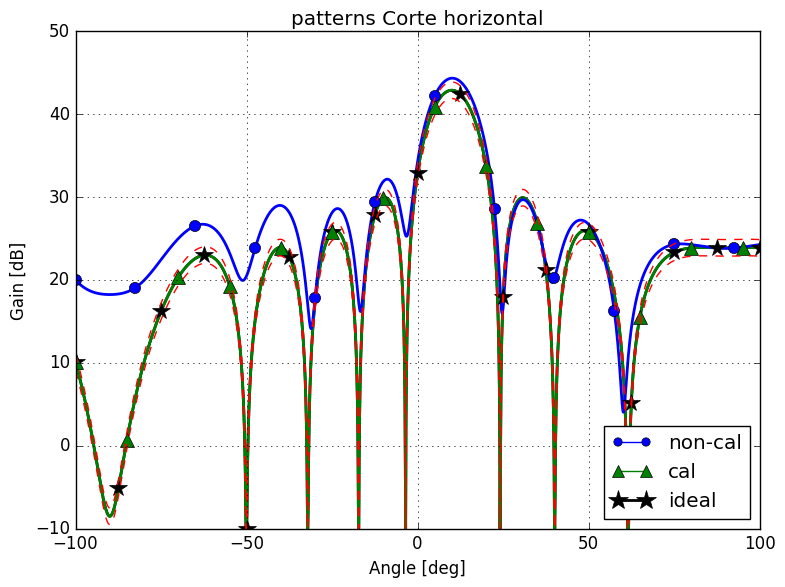
\includegraphics[width=7cm]{gfx/compErrMutual10degColAzCut.png}}
 	\subfloat[]{
		\includegraphics[width=7cm]{gfx/compErrMutual10degColElCut.png}}
	\caption{Correcciones de la señal transmitida utilizando calibración por acoplamientos mutuos. (a) ganancia y fase 
		transmitida por módulos radiantes. (b) corte horizontal del diagrama transmitido y (c) corte vertical del diagrama transmitido.}
	\label{fig:compErrMutual10degCol}
\end{figure}

\begin{table}[H]
  \footnotesize
  \centering
  \begin{tabular}{|c|c|p{2cm}|p{2.5cm}|p{2.5cm}|p{2.5cm}|}
    \cline{2-6}
    \multicolumn{1}{c|}{} & Corte & Ganancia - lóbulo izq. [dBc] & Ganancia - lóbulo central [dB] &
    Ganancia - lóbulo der. [dBc] & Ancho - lóbulo central -3dB \tabularnewline\hline
    \multirow{2}{2cm}{Pat. sin calibrar} & H & 14.68 & 42.56 & 13.86 & 13.0 \tabularnewline\cline{2-6}
     & V & 7.37 & 34.13 & 11.18 & 16.4 \tabularnewline\hline
    \multirow{2}{2cm}{Pat. calibrado} & H & 12.97 & 42.9 & 12.97 & 12.4 \tabularnewline\cline{2-6}
     & V & 12.65 & 32.96 & 12.65 & 17.4 \tabularnewline\hline
    \multirow{2}{2cm}{Pat. ideal} & H & 12.97 & 42.9 & 12.97 & 12.4 \tabularnewline\cline{2-6}
     & V & 12.65 & 32.96 & 12.65 & 17.4 \tabularnewline\hline
    \multirow{2}{2cm}{Dif. sin calibrar} & H & 1.71 & -0.34 & 0.89 & 0.6\tabularnewline\cline{2-6}
     & V & -5.28 & 1.17 & -1.47 & -1.0 \tabularnewline\hline
    \multirow{2}{2cm}{Dif. calibrado} & H & 0.0 & 0.0 & 0.0 & 0.0 \tabularnewline\cline{2-6}
     & V & 0.0 & 0.0 & 0.0 & 0.0 \tabularnewline\hline
  \end{tabular}
  \caption{Propiedades de los patrones calibrados y sin calibrar comparados con el ideal.}
  \label{tab:compErrMutual10degCol}
\end{table}


\subsubsection{Apuntamiento 10 grados en dirección vertical}

Los gráficos de la figura \ref{fig:compErrMutual10degRow} muestran que el calibrador funciona correctamente y que los diagramas de 
radiación de la señal calibrada se asemejan al ideal. 

\begin{figure}[H]
	\centering
 	\subfloat[]{
		\includegraphics[width=9cm]{gfx/compErrMutual10degRow.png}}

	\subfloat[]{
		\includegraphics[width=7cm]{gfx/compErrMutual10degRowAzCut.png}}
 	\subfloat[]{
		\includegraphics[width=7cm]{gfx/compErrMutual10degRowElCut.png}}
	\caption{Correcciones de la señal transmitida utilizando calibración por acoplamientos mutuos. (a) ganancia y fase 
		transmitida por módulos radiantes. (b) corte horizontal del diagrama transmitido y (c) corte vertical del diagrama transmitido.}
	\label{fig:compErrMutual10degRow}
\end{figure}

La tabla \ref{tab:compErrMutual10degRow} muestra que las diferencias de ganacia de los lóbulos secundarios entre los diagramas 
reales y el ideal para ambos cortes están dentro de la máscara admisible. A su vez, también se observa la mejora en el ancho 
del lóbulo principal. 

\begin{table}[H]
  \footnotesize
  \centering
  \begin{tabular}{|c|c|p{2cm}|p{2.5cm}|p{2.5cm}|p{2.5cm}|}
    \cline{2-6}
    \multicolumn{1}{c|}{} & Corte & Ganancia - lóbulo izq. [dBc] & Ganancia - lóbulo central [dB] &
    Ganancia - lóbulo der. [dBc] & Ancho - lóbulo central -3dB \tabularnewline\hline
    \multirow{2}{2cm}{Pat. sin calibrar} & H & 10.36 & 39.16 & 18.48 & 13.0 \tabularnewline\cline{2-6}
     & V & 7.74 & 42.97 & 7.35 & 16.8 \tabularnewline\hline
    \multirow{2}{2cm}{Pat. calibrado} & H & 12.78 & 38.78 & 13.01 & 12.0 \tabularnewline\cline{2-6}
     & V & 12.57 & 42.9 & 12.71 & 17.8 \tabularnewline\hline
    \multirow{2}{2cm}{Pat. ideal} & H & 12.97 & 38.76 & 12.97 & 12.0 \tabularnewline\cline{2-6}
     & V & 12.65 & 42.9 & 12.65 & 17.8 \tabularnewline\hline
    \multirow{2}{2cm}{Dif. sin calibrar} & H & -2.61 & 0.4 & 5.51 & 1.0\tabularnewline\cline{2-6}
     & V & -4.91 & 0.07 & -5.3 & -1.0 \tabularnewline\hline
    \multirow{2}{2cm}{Dif. calibrado} & H & -0.19 & 0.02 & 0.04 & 0.0 \tabularnewline\cline{2-6}
     & V & -0.08 & 0.0 & 0.06 & 0.0 \tabularnewline\hline
  \end{tabular}
  \caption{Propiedades de los patrones calibrados y sin calibrar comparados con el ideal.}
  \label{tab:compErrMutual10degRow}
\end{table}


\section{Dispersiones de ganancia entre pulsos}

En esta sección se agregan dispersiones de fase y ganancia en el generador de la señal utilizada para transmitir y calibrar 
la antena. Las otras características de este ensayo son:
\begin{itemize}
	\item Desvío estándar en ganancia de 1 dB entre pulsos de calibración.
	\item Desvío estándar en fase de 5 grados entre pulsos de calibración
	\item No hay dispersiones en el comportamiento de los componentes de la antena.
	\item No hay errores de calibración.
\end{itemize}

\subsection{Utilizando la calibración clásica}

\subsubsection{Apuntamiento uniforme}

En las imágenes de la figura \ref{fig:chirpErrClassical0deg} se puede apreciar como, sacando de lado la diferencia de 
ganancia y fase por no abarcar la completitud del sistema, esta incertidumbre hace que el calibrador no funcione correctamente 
ni para medir fase ni ganancias de cada elemento, introduciendo diferencias de hasta 25 dBs en ganancia y 100 grados en fase.
A su vez, se puede observar que los diagramas de radiación están defasados en ganancia por mucho.

En la tabla \ref{tab:chirpErrClassical0deg} se pueden apreciar que si bien las ganancias de los lóbulos principales es muy 
diferente, rondando los 24 dBs, los diagramas de radiación ya poseen lóbulos segundarios mayores al permitido por medio dB. El 
ancho del lóbulo principal también se ve afectado, resultando en 1 grado mayor.

\begin{figure}[H]
	\centering
 	\subfloat[]{
		\includegraphics[width=9cm]{gfx/chirpErrClassical0deg.png}}

	\subfloat[]{
		\includegraphics[width=7cm]{gfx/chirpErrClassical0degAzCut.png}}
 	\subfloat[]{
		\includegraphics[width=7cm]{gfx/chirpErrClassical0degElCut.png}}
	\caption{Correcciones de la señal transmitida utilizando calibración clásica. (a) ganancia y fase transmitida por módulos
		radiantes. (b) corte horizontal del diagrama transmitido y (c) corte vertical del diagrama transmitido.}
	\label{fig:chirpErrClassical0deg}
\end{figure}

\begin{table}[H]
  \footnotesize
  \centering
  \begin{tabular}{|c|c|p{2cm}|p{2.5cm}|p{2.5cm}|p{2.5cm}|}
    \cline{2-6}
    \multicolumn{1}{c|}{} & Corte & Ganancia - lóbulo izq. [dBc] & Ganancia - lóbulo central [dB] &
    Ganancia - lóbulo der. [dBc] & Ancho - lóbulo central -3dB \tabularnewline\hline
    \multirow{2}{2cm}{Pat. sin calibrar} & H & 12.97 & 43.48 & 12.97 & 12.0 \tabularnewline\cline{2-6}
     & V & 12.65 & 43.48 & 12.65 & 17.4 \tabularnewline\hline
    \multirow{2}{2cm}{Pat. calibrado} & H & 13.9 & 34.49 & 14.1 & 12.2 \tabularnewline\cline{2-6}
     & V & 16.14 & 34.49 & 16.88 & 17.8 \tabularnewline\hline
    \multirow{2}{2cm}{Pat. ideal} & H & 12.97 & 42.9 & 12.97 & 12.0 \tabularnewline\cline{2-6}
     & V & 12.65 & 42.9 & 12.65 & 17.4 \tabularnewline\hline
    \multirow{2}{2cm}{Dif. sin calibrar} & H & 0.0 & 0.58 & 0.0 & 0.0\tabularnewline\cline{2-6}
     & V & 0.0 & 0.58 & 0.0 & 0.0 \tabularnewline\hline
    \multirow{2}{2cm}{Dif. calibrado} & H & 0.93 & -8.41 & 1.13 & 0.2 \tabularnewline\cline{2-6}
     & V & 3.49 & -8.41 & 4.23 & 0.4 \tabularnewline\hline
  \end{tabular}
  \caption{Propiedades de los patrones calibrados y sin calibrar comparados con el ideal.}
  \label{tab:chirpErrClassical0deg}
\end{table}


\subsubsection{Apuntamiento 10 grados en dirección horizontal}

En las imágenes de la figura \ref{fig:chirpErrClassical10degCol} se puede apreciar como, sacando de lado la diferencia de 
ganancia y fase por no abarcar la completitud del sistema, esta incertidumbre hace que el calibrador no funcione correctamente 
ni para medir fase ni ganancias de cada elemento, introduciendo diferencias de hasta 15 dBs en ganancia y 70 grados en fase. 
A su vez, se puede observar que los diagramas de radiación poseen lóbulos secundarios con una ganancia mucho mayor a la aceptada.

En la tabla \ref{tab:chirpErrClassical10degCol} se pueden apreciar que si bien las ganancias de los lóbulos principales son 
diferentes por 1.5 dBs, las diferencias por los lóbulos secundarios rondan los 7 dB. El ancho del lóbulo principal también 
se ve afectado, resultando en aproximadamente 1 grado mayor.

\begin{figure}[H]
	\centering
 	\subfloat[]{
		\includegraphics[width=9cm]{gfx/chirpErrClassical10degCol.png}}

	\subfloat[]{
		\includegraphics[width=7cm]{gfx/chirpErrClassical10degColAzCut.png}}
 	\subfloat[]{
		\includegraphics[width=7cm]{gfx/chirpErrClassical10degColElCut.png}}
	\caption{Correcciones de la señal transmitida utilizando calibración clásica. (a) ganancia y fase transmitida por módulos
		radiantes. (b) corte horizontal del diagrama transmitido y (c) corte vertical del diagrama transmitido.}
	\label{fig:chirpErrClassical10degCol}
\end{figure}

\begin{table}[H]
  \footnotesize
  \centering
  \begin{tabular}{|c|c|p{2cm}|p{2.5cm}|p{2.5cm}|p{2.5cm}|}
    \cline{2-6}
    \multicolumn{1}{c|}{} & Corte & Ganancia - lóbulo izq. [dBc] & Ganancia - lóbulo central [dB] &
    Ganancia - lóbulo der. [dBc] & Ancho - lóbulo central -3dB \tabularnewline\hline
    \multirow{2}{2cm}{Pat. sin calibrar} & H & 12.97 & 43.48 & 12.97 & 12.4 \tabularnewline\cline{2-6}
     & V & 12.65 & 33.54 & 12.65 & 17.4 \tabularnewline\hline
    \multirow{2}{2cm}{Pat. calibrado} & H & 14.51 & 37.86 & 12.43 & 13.2 \tabularnewline\cline{2-6}
     & V & 4.02 & 25.0 & 25.0 & 0 \tabularnewline\hline
    \multirow{2}{2cm}{Pat. ideal} & H & 12.97 & 42.9 & 12.97 & 12.4 \tabularnewline\cline{2-6}
     & V & 12.65 & 32.96 & 12.65 & 17.4 \tabularnewline\hline
    \multirow{2}{2cm}{Dif. sin calibrar} & H & 0.0 & 0.58 & 0.0 & 0.0\tabularnewline\cline{2-6}
     & V & 0.0 & 0.58 & 0.0 & 0.0 \tabularnewline\hline
    \multirow{2}{2cm}{Dif. calibrado} & H & 1.54 & -5.04 & -0.54 & 0.8 \tabularnewline\cline{2-6}
     & V & -8.63 & -7.96 & 12.35 & -17.4 \tabularnewline\hline
  \end{tabular}
  \caption{Propiedades de los patrones calibrados y sin calibrar comparados con el ideal.}
  \label{tab:chirpErrClassical10degCol}
\end{table}


\subsubsection{Apuntamiento 10 grados en dirección vertical}

En las imágenes de la figura \ref{fig:chirpErrClassical10degRow} se puede apreciar como, sacando de lado la diferencia de 
ganancia y fase por no abarcar la completitud del sistema, esta incertidumbre hace que el calibrador no funcione correctamente 
ni para medir fase ni ganancias de cada elemento, introduciendo diferencias de hasta 15 dBs en ganancia y 70 grados en fase. 
A su vez, se puede observar que los diagramas de radiación poseen lóbulos secundarios con una ganancia mucho mayor a la aceptada.

En la tabla \ref{tab:chirpErrClassical10degRow} se pueden apreciar que si bien las ganancias de los lóbulos principales son 
diferentes por 1.5 dBs, las diferencias por los lóbulos secundarios rondan los 5 dB. El ancho del lóbulo principal también 
se ve afectado, resultando en aproximadamente 0.6 grados mayor.

\begin{figure}[H]
	\centering
 	\subfloat[]{
		\includegraphics[width=9cm]{gfx/chirpErrClassical10degRow.png}}

	\subfloat[]{
		\includegraphics[width=7cm]{gfx/chirpErrClassical10degRowAzCut.png}}
 	\subfloat[]{
		\includegraphics[width=7cm]{gfx/chirpErrClassical10degRowElCut.png}}
	\caption{Correcciones de la señal transmitida utilizando calibración clásica. (a) ganancia y fase transmitida por módulos
		radiantes. (b) corte horizontal del diagrama transmitido y (c) corte vertical del diagrama transmitido.}
	\label{fig:chirpErrClassical10degRow}
\end{figure}

\begin{table}[H]
  \footnotesize
  \centering
  \begin{tabular}{|c|c|p{2cm}|p{2.5cm}|p{2.5cm}|p{2.5cm}|}
    \cline{2-6}
    \multicolumn{1}{c|}{} & Corte & Ganancia - lóbulo izq. [dBc] & Ganancia - lóbulo central [dB] &
    Ganancia - lóbulo der. [dBc] & Ancho - lóbulo central -3dB \tabularnewline\hline
    \multirow{2}{2cm}{Pat. sin calibrar} & H & 12.97 & 39.34 & 12.97 & 12.0 \tabularnewline\cline{2-6}
     & V & 12.65 & 43.48 & 12.65 & 17.8 \tabularnewline\hline
    \multirow{2}{2cm}{Pat. calibrado} & H & 10.89 & 32.8 & 7.99 & 12.4 \tabularnewline\cline{2-6}
     & V & 0.32 & 39.05 & 39.05 & 0 \tabularnewline\hline
    \multirow{2}{2cm}{Pat. ideal} & H & 12.97 & 38.76 & 12.97 & 12.0 \tabularnewline\cline{2-6}
     & V & 12.65 & 42.9 & 12.65 & 17.8 \tabularnewline\hline
    \multirow{2}{2cm}{Dif. sin calibrar} & H & 0.0 & 0.58 & 0.0 & 0.0\tabularnewline\cline{2-6}
     & V & 0.0 & 0.58 & 0.0 & 0.0 \tabularnewline\hline
    \multirow{2}{2cm}{Dif. calibrado} & H & -2.08 & -5.96 & -4.98 & 0.4 \tabularnewline\cline{2-6}
     & V & -12.33 & -3.85 & 26.4 & -17.8 \tabularnewline\hline
  \end{tabular}
  \caption{Propiedades de los patrones calibrados y sin calibrar comparados con el ideal.}
  \label{tab:chirpErrClassical10degRow}
\end{table}


\subsection{Utilizando la calibración con acoplamientos mútuos}

\subsubsection{Apuntamiento uniforme}

En las imágenes de la figura \ref{fig:chirpErrMutual0deg} se puede apreciar como esta incertidumbre hace que el calibrador 
no funcione tan correctamente ni para medir fase ni ganancias de cada elemento, introduciendo diferencias de hasta 3 dBs en 
ganancia y 6 grados en fase. A su vez, se puede observar que, independientemente de este desvío introducido, los diagramas de 
radiación se mantienen cerca del esperado, salvo por la ganancia esperada.

En la tabla \ref{tab:chirpErrMutual0deg} se pueden apreciar que si bien las ganancias de los lóbulos principales son 
diferentes por máximo 2 dBs, las diferencias por los lóbulos secundarios rondan los 0.1 dB. Se puede concluir que el 
calibrador es bastante robusto frente a esta clase de incertidumbres. El ancho del lóbulo principal también se ve afectado,
resultando en aproximadamente 0.2 grados mayor.

\begin{figure}[H]
	\centering
 	\subfloat[]{
		\includegraphics[width=9cm]{gfx/chirpErrMutual0deg.png}}

	\subfloat[]{
		\includegraphics[width=7cm]{gfx/chirpErrMutual0degAzCut.png}}
 	\subfloat[]{
		\includegraphics[width=7cm]{gfx/chirpErrMutual0degElCut.png}}
	\caption{Correcciones de la señal transmitida utilizando calibración por acoplamientos mutuos. (a) ganancia y fase transmitida por módulos
		radiantes. (b) corte horizontal del diagrama transmitido y (c) corte vertical del diagrama transmitido.}
	\label{fig:chirpErrMutual0deg}
\end{figure}

\begin{table}[H]
  \footnotesize
  \centering
  \begin{tabular}{|c|c|p{2cm}|p{2.5cm}|p{2.5cm}|p{2.5cm}|}
    \cline{2-6}
    \multicolumn{1}{c|}{} & Corte & Ganancia - lóbulo izq. [dBc] & Ganancia - lóbulo central [dB] &
    Ganancia - lóbulo der. [dBc] & Ancho - lóbulo central -3dB \tabularnewline\hline
    \multirow{2}{2cm}{Pat. sin calibrar} & H & 12.97 & 43.48 & 12.97 & 12.0 \tabularnewline\cline{2-6}
     & V & 12.65 & 43.48 & 12.65 & 17.4 \tabularnewline\hline
    \multirow{2}{2cm}{Pat. calibrado} & H & 13.13 & 40.94 & 12.92 & 12.2 \tabularnewline\cline{2-6}
     & V & 12.7 & 40.94 & 12.74 & 17.4 \tabularnewline\hline
    \multirow{2}{2cm}{Pat. ideal} & H & 12.97 & 42.9 & 12.97 & 12.0 \tabularnewline\cline{2-6}
     & V & 12.65 & 42.9 & 12.65 & 17.4 \tabularnewline\hline
    \multirow{2}{2cm}{Dif. sin calibrar} & H & 0.0 & 0.58 & 0.0 & 0.0\tabularnewline\cline{2-6}
     & V & 0.0 & 0.58 & 0.0 & 0.0 \tabularnewline\hline
    \multirow{2}{2cm}{Dif. calibrado} & H & 0.16 & -1.96 & -0.05 & 0.2 \tabularnewline\cline{2-6}
     & V & 0.05 & -1.96 & 0.09 & 0.0 \tabularnewline\hline
  \end{tabular}
  \caption{Propiedades de los patrones calibrados y sin calibrar comparados con el ideal.}
  \label{tab:chirpErrMutual0deg}
\end{table}


\subsubsection{Apuntamiento 10 grados en dirección horizontal}

En las imágenes de la figura \ref{fig:chirpErrMutual10degCol} se puede apreciar como esta incertidumbre hace que el calibrador 
no funcione tan correctamente ni para medir fase ni ganancias de cada elemento, introduciendo diferencias de hasta 1.4 dBs en 
ganancia y unos pocos grados en fase. A su vez, se puede observar que, independientemente de este desvío introducido, los diagramas de 
radiación se mantienen cerca del esperado.

En la tabla \ref{tab:chirpErrMutual10degCol} se pueden apreciar que, tanto las ganancias de los lóbulos principales como la de 
los lóbulos secundarios, se mantiene dentro de la máscara permitida. Se puede concluir que el calibrador es bastante robusto 
frente a esta clase de incertidumbres. El ancho del lóbulo principal también se ve afectado, resultando en aproximadamente 0.2
grados mayor.

\begin{figure}[H]
	\centering
 	\subfloat[]{
		\includegraphics[width=9cm]{gfx/chirpErrMutual10degCol.png}}

	\subfloat[]{
		\includegraphics[width=7cm]{gfx/chirpErrMutual10degColAzCut.png}}
 	\subfloat[]{
		\includegraphics[width=7cm]{gfx/chirpErrMutual10degColElCut.png}}
	\caption{Correcciones de la señal transmitida utilizando calibración por acoplamientos mutuos. (a) ganancia y fase 
		transmitida por módulos radiantes. (b) corte horizontal del diagrama transmitido y (c) corte vertical del diagrama transmitido.}
	\label{fig:chirpErrMutual10degCol}
\end{figure}

\begin{table}[H]
  \footnotesize
  \centering
  \begin{tabular}{|c|c|p{2cm}|p{2.5cm}|p{2.5cm}|p{2.5cm}|}
    \cline{2-6}
    \multicolumn{1}{c|}{} & Corte & Ganancia - lóbulo izq. [dBc] & Ganancia - lóbulo central [dB] &
    Ganancia - lóbulo der. [dBc] & Ancho - lóbulo central -3dB \tabularnewline\hline
    \multirow{2}{2cm}{Pat. sin calibrar} & H & 12.97 & 43.48 & 12.97 & 12.4 \tabularnewline\cline{2-6}
     & V & 12.65 & 33.54 & 12.65 & 17.4 \tabularnewline\hline
    \multirow{2}{2cm}{Pat. calibrado} & H & 13.11 & 42.58 & 13.03 & 12.6 \tabularnewline\cline{2-6}
     & V & 12.7 & 32.61 & 12.86 & 17.4 \tabularnewline\hline
    \multirow{2}{2cm}{Pat. ideal} & H & 12.97 & 42.9 & 12.97 & 12.4 \tabularnewline\cline{2-6}
     & V & 12.65 & 32.96 & 12.65 & 17.4 \tabularnewline\hline
    \multirow{2}{2cm}{Dif. sin calibrar} & H & 0.0 & 0.58 & 0.0 & 0.0\tabularnewline\cline{2-6}
     & V & 0.0 & 0.58 & 0.0 & 0.0 \tabularnewline\hline
    \multirow{2}{2cm}{Dif. calibrado} & H & 0.14 & -0.32 & 0.06 & 0.2 \tabularnewline\cline{2-6}
     & V & 0.05 & -0.35 & 0.21 & 0.0 \tabularnewline\hline
  \end{tabular}
  \caption{Propiedades de los patrones calibrados y sin calibrar comparados con el ideal.}
  \label{tab:chirpErrMutual10degCol}
\end{table}


\subsubsection{Apuntamiento 10 grados en dirección vertical}

En las imágenes de la figura \ref{fig:chirpErrMutual10degRow} se puede apreciar como esta incertidumbre hace que el calibrador 
no funcione tan correctamente ni para medir fase ni ganancias de cada elemento, introduciendo diferencias de hasta 1.6 dBs en 
ganancia y unos pocos grados en fase. A su vez, se puede observar que, independientemente de este desvío introducido, los diagramas de 
radiación se mantienen cerca del esperado.

En la tabla \ref{tab:chirpErrMutual10degRow} se pueden apreciar que, tanto las ganancias de los lóbulos principales como la de 
los lóbulos secundarios, se mantiene dentro de la máscara permitida. Se puede concluir que el calibrador es bastante robusto 
frente a esta clase de incertidumbres. El ancho del lóbulo principal también se ve afectado, resultando en aproximadamente 0.2
grados mayor.

\begin{figure}[H]
	\centering
 	\subfloat[]{
		\includegraphics[width=9cm]{gfx/chirpErrMutual10degRow.png}}

	\subfloat[]{
		\includegraphics[width=7cm]{gfx/chirpErrMutual10degRowAzCut.png}}
 	\subfloat[]{
		\includegraphics[width=7cm]{gfx/chirpErrMutual10degRowElCut.png}}
	\caption{Correcciones de la señal transmitida utilizando calibración por acoplamientos mutuos. (a) ganancia y fase 
		transmitida por módulos radiantes. (b) corte horizontal del diagrama transmitido y (c) corte vertical del diagrama transmitido.}
	\label{fig:chirpErrMutual10degRow}
\end{figure}

\begin{table}[H]
  \footnotesize
  \centering
  \begin{tabular}{|c|c|p{2cm}|p{2.5cm}|p{2.5cm}|p{2.5cm}|}
    \cline{2-6}
    \multicolumn{1}{c|}{} & Corte & Ganancia - lóbulo izq. [dBc] & Ganancia - lóbulo central [dB] &
    Ganancia - lóbulo der. [dBc] & Ancho - lóbulo central -3dB \tabularnewline\hline
    \multirow{2}{2cm}{Pat. sin calibrar} & H & 12.97 & 39.34 & 12.97 & 12.0 \tabularnewline\cline{2-6}
     & V & 12.65 & 43.48 & 12.65 & 17.8 \tabularnewline\hline
    \multirow{2}{2cm}{Pat. calibrado} & H & 13.06 & 39.28 & 12.66 & 12.2 \tabularnewline\cline{2-6}
     & V & 12.55 & 43.44 & 12.61 & 17.8 \tabularnewline\hline
    \multirow{2}{2cm}{Pat. ideal} & H & 12.97 & 38.76 & 12.97 & 12.0 \tabularnewline\cline{2-6}
     & V & 12.65 & 42.9 & 12.65 & 17.8 \tabularnewline\hline
    \multirow{2}{2cm}{Dif. sin calibrar} & H & 0.0 & 0.58 & 0.0 & 0.0\tabularnewline\cline{2-6}
     & V & 0.0 & 0.58 & 0.0 & 0.0 \tabularnewline\hline
    \multirow{2}{2cm}{Dif. calibrado} & H & 0.09 & 0.52 & -0.31 & 0.2 \tabularnewline\cline{2-6}
     & V & -0.1 & 0.54 & -0.04 & 0.0 \tabularnewline\hline
  \end{tabular}
  \caption{Propiedades de los patrones calibrados y sin calibrar comparados con el ideal.}
  \label{tab:chirpErrMutual10degRow}
\end{table}


\section{Dispersión de ganancia de la chirp réplica}

Como la chirp réplica es simplemente utilizada en la calibración clásica, en esta simulación no se podrán comparar 
resultados, pero sirve para determinar que tan robusto es el método para esta clase de errores. Por como funciona el método, 
se espera un defasaje en la caracterización igual para todos los elementos tanto en ganancia como en fase. El desvío estándar
utilizado es de 1dB para la ganancia y 5 grados para la fase.

\subsection{Apuntamiento uniforme}

En las imágenes de la figura \ref{fig:chirpRepErrClassical0deg} se puede apreciar como, sacando de lado la diferencia de 
ganancia y fase por no abarcar la completitud del sistema, la ganancia y fase de cada elemento radiante posee un defasaje con 
respecto al valor ideal mayor a la señal no calibrada. De todas formas, es importante resaltar que el diagrama de radiación no 
se deforma. 

En la tabla \ref{tab:chirpRepErrClassical0deg} se pueden apreciar que realmente no hay diferencias en los lóbulos secundarios 
ni en el ancho del lóbulo principal. Si es apreciable la diferencia en ganancia de todo el diagrama de radiación.

\begin{figure}[H]
	\centering
 	\subfloat[]{
		\includegraphics[width=9cm]{gfx/chirpRepErrClassical0deg.png}}

	\subfloat[]{
		\includegraphics[width=7cm]{gfx/chirpRepErrClassical0degAzCut.png}}
 	\subfloat[]{
		\includegraphics[width=7cm]{gfx/chirpRepErrClassical0degElCut.png}}
	\caption{Correcciones de la señal transmitida utilizando calibración clásica. (a) ganancia y fase transmitida por módulos
		radiantes. (b) corte horizontal del diagrama transmitido y (c) corte vertical del diagrama transmitido.}
	\label{fig:chirpRepErrClassical0deg}
\end{figure}

\begin{table}[H]
  \footnotesize
  \centering
  \begin{tabular}{|c|c|p{2cm}|p{2.5cm}|p{2.5cm}|p{2.5cm}|}
    \cline{2-6}
    \multicolumn{1}{c|}{} & Corte & Ganancia - lóbulo izq. [dBc] & Ganancia - lóbulo central [dB] &
    Ganancia - lóbulo der. [dBc] & Ancho - lóbulo central -3dB \tabularnewline\hline
    \multirow{2}{2cm}{Pat. sin calibrar} & H & 12.97 & 43.48 & 12.97 & 12.0 \tabularnewline\cline{2-6}
     & V & 12.65 & 43.48 & 12.65 & 17.4 \tabularnewline\hline
    \multirow{2}{2cm}{Pat. calibrado} & H & 12.97 & 36.8 & 12.97 & 12.0 \tabularnewline\cline{2-6}
     & V & 12.65 & 36.8 & 12.65 & 17.4 \tabularnewline\hline
    \multirow{2}{2cm}{Pat. ideal} & H & 12.97 & 42.9 & 12.97 & 12.0 \tabularnewline\cline{2-6}
     & V & 12.65 & 42.9 & 12.65 & 17.4 \tabularnewline\hline
    \multirow{2}{2cm}{Dif. sin calibrar} & H & 0.0 & 0.58 & 0.0 & 0.0\tabularnewline\cline{2-6}
     & V & 0.0 & 0.58 & 0.0 & 0.0 \tabularnewline\hline
    \multirow{2}{2cm}{Dif. calibrado} & H & 0.0 & -6.1 & 0.0 & 0.0 \tabularnewline\cline{2-6}
     & V & 0.0 & -6.1 & 0.0 & 0.0 \tabularnewline\hline
  \end{tabular}
  \caption{Propiedades de los patrones calibrados y sin calibrar comparados con el ideal.}
  \label{tab:chirpRepErrClassical0deg}
\end{table}


\subsection{Apuntamiento 10 grados en dirección horizontal}

En las imágenes de la figura \ref{fig:chirpRepErrClassical10degCol} se puede apreciar como, sacando de lado la diferencia de 
ganancia y fase por no abarcar la completitud del sistema, la ganancia y fase de cada elemento radiante posee un defasaje con 
respecto al valor ideal mayor a la señal no calibrada. De todas formas, es importante resaltar que el diagrama de radiación no 
se deforma. 

En la tabla \ref{tab:chirpRepErrClassical10degCol} se pueden apreciar que realmente no hay diferencias en los lóbulos secundarios 
ni en el ancho del lóbulo principal. Si es apreciable la diferencia en ganancia de todo el diagrama de radiación.

\begin{figure}[H]
	\centering
 	\subfloat[]{
		\includegraphics[width=9cm]{gfx/chirpRepErrClassical10degCol.png}}

	\subfloat[]{
		\includegraphics[width=7cm]{gfx/chirpRepErrClassical10degColAzCut.png}}
 	\subfloat[]{
		\includegraphics[width=7cm]{gfx/chirpRepErrClassical10degColElCut.png}}
	\caption{Correcciones de la señal transmitida utilizando calibración clásica. (a) ganancia y fase transmitida por módulos
		radiantes. (b) corte horizontal del diagrama transmitido y (c) corte vertical del diagrama transmitido.}
	\label{fig:chirpRepErrClassical10degCol}
\end{figure}

\begin{table}[H]
  \footnotesize
  \centering
  \begin{tabular}{|c|c|p{2cm}|p{2.5cm}|p{2.5cm}|p{2.5cm}|}
    \cline{2-6}
    \multicolumn{1}{c|}{} & Corte & Ganancia - lóbulo izq. [dBc] & Ganancia - lóbulo central [dB] &
    Ganancia - lóbulo der. [dBc] & Ancho - lóbulo central -3dB \tabularnewline\hline
    \multirow{2}{2cm}{Pat. sin calibrar} & H & 12.97 & 43.48 & 12.97 & 12.4 \tabularnewline\cline{2-6}
     & V & 12.65 & 33.54 & 12.65 & 17.4 \tabularnewline\hline
    \multirow{2}{2cm}{Pat. calibrado} & H & 12.97 & 36.8 & 12.97 & 12.4 \tabularnewline\cline{2-6}
     & V & 12.65 & 26.86 & 12.65 & 17.4 \tabularnewline\hline
    \multirow{2}{2cm}{Pat. ideal} & H & 12.97 & 42.9 & 12.97 & 12.4 \tabularnewline\cline{2-6}
     & V & 12.65 & 32.96 & 12.65 & 17.4 \tabularnewline\hline
    \multirow{2}{2cm}{Dif. sin calibrar} & H & 0.0 & 0.58 & 0.0 & 0.0\tabularnewline\cline{2-6}
     & V & 0.0 & 0.58 & 0.0 & 0.0 \tabularnewline\hline
    \multirow{2}{2cm}{Dif. calibrado} & H & 0.0 & -6.1 & 0.0 & 0.0 \tabularnewline\cline{2-6}
     & V & 0.0 & -6.1 & 0.0 & 0.0 \tabularnewline\hline
  \end{tabular}
  \caption{Propiedades de los patrones calibrados y sin calibrar comparados con el ideal.}
  \label{tab:chirpRepErrClassical10degCol}
\end{table}


\subsection{Apuntamiento 10 grados en dirección vertical}

En las imágenes de la figura \ref{fig:chirpRepErrClassical10degCol} se puede apreciar como, sacando de lado la diferencia de 
ganancia y fase por no abarcar la completitud del sistema, la ganancia y fase de cada elemento radiante posee un defasaje con 
respecto al valor ideal mayor a la señal no calibrada. De todas formas, es importante resaltar que el diagrama de radiación no 
se deforma. 

En la tabla \ref{tab:chirpRepErrClassical10degCol} se pueden apreciar que realmente no hay diferencias en los lóbulos secundarios 
ni en el ancho del lóbulo principal. Si es apreciable la diferencia en ganancia de todo el diagrama de radiación.

\begin{figure}[H]
	\centering
 	\subfloat[]{
		\includegraphics[width=9cm]{gfx/chirpRepErrClassical10degRow.png}}

	\subfloat[]{
		\includegraphics[width=7cm]{gfx/chirpRepErrClassical10degRowAzCut.png}}
 	\subfloat[]{
		\includegraphics[width=7cm]{gfx/chirpRepErrClassical10degRowElCut.png}}
	\caption{Correcciones de la señal transmitida utilizando calibración clásica. (a) ganancia y fase transmitida por módulos
		radiantes. (b) corte horizontal del diagrama transmitido y (c) corte vertical del diagrama transmitido.}
	\label{fig:chirpRepErrClassical10degRow}
\end{figure}

\begin{table}[H]
  \footnotesize
  \centering
  \begin{tabular}{|c|c|p{2cm}|p{2.5cm}|p{2.5cm}|p{2.5cm}|}
    \cline{2-6}
    \multicolumn{1}{c|}{} & Corte & Ganancia - lóbulo izq. [dBc] & Ganancia - lóbulo central [dB] &
    Ganancia - lóbulo der. [dBc] & Ancho - lóbulo central -3dB \tabularnewline\hline
    \multirow{2}{2cm}{Pat. sin calibrar} & H & 12.97 & 39.34 & 12.97 & 12.0 \tabularnewline\cline{2-6}
     & V & 12.65 & 43.48 & 12.65 & 17.8 \tabularnewline\hline
    \multirow{2}{2cm}{Pat. calibrado} & H & 12.97 & 32.65 & 12.97 & 12.0 \tabularnewline\cline{2-6}
     & V & 12.65 & 36.8 & 12.65 & 17.8 \tabularnewline\hline
    \multirow{2}{2cm}{Pat. ideal} & H & 12.97 & 38.76 & 12.97 & 12.0 \tabularnewline\cline{2-6}
     & V & 12.65 & 42.9 & 12.65 & 17.8 \tabularnewline\hline
    \multirow{2}{2cm}{Dif. sin calibrar} & H & 0.0 & 0.58 & 0.0 & 0.0\tabularnewline\cline{2-6}
     & V & 0.0 & 0.58 & 0.0 & 0.0 \tabularnewline\hline
    \multirow{2}{2cm}{Dif. calibrado} & H & 0.0 & -6.11 & 0.0 & 0.0 \tabularnewline\cline{2-6}
     & V & 0.0 & -6.1 & 0.0 & 0.0 \tabularnewline\hline
  \end{tabular}
  \caption{Propiedades de los patrones calibrados y sin calibrar comparados con el ideal.}
  \label{tab:chirpRepErrClassical10degRow}
\end{table}


\section{Dispersión de fase del Walsh}

Como los códigos walsh son solamente utilizados en la calibración clásica, en esta simulación no se podrán comparar 
resultados, pero sirve para determinar que tan robusto es el método para esta clase de errores. 

Esots desvíos serían en la configuración de los $\pm 90$ grados de los defasadores a la hora de realizar la calibración con 
el método clásico. El desvío estándar utilizado es de 5 grados. 

\subsection{Apuntamiento uniforme}

En las imágenes de la figura \ref{fig:wallErrClassical0deg} se puede apreciar como, sacando de lado la diferencia de ganancia 
y fase por no abarcar la completitud del sistema, la señal calibrada resulta ser distorsionada por el efecto que los códigos 
resultantes dejan de ser completamente ortogonales entre sí. Es importante notar que esta clase de desvíos genera mayores 
variaciones en la ganancia de los elementos que en la fase de los mismos.

En la tabla \ref{tab:wallErrClassical0deg} se pueden apreciar las diferencias generadas por esta clase de dispersión, los 
lóbulos secundarios del diagrama de radiación calibrado se diferencia del ideal por una maginitud que ronda los 0.3 dBs. El 
lóbulo principal se ensancha en 0.2 grados.

\begin{figure}[H]
	\centering
 	\subfloat[]{
		\includegraphics[width=9cm]{gfx/wallErrClassical0deg.png}}

	\subfloat[]{
		\includegraphics[width=7cm]{gfx/wallErrClassical0degAzCut.png}}
 	\subfloat[]{
		\includegraphics[width=7cm]{gfx/wallErrClassical0degElCut.png}}
	\caption{Correcciones de la señal transmitida utilizando calibración clásica. (a) ganancia y fase transmitida por módulos
		radiantes. (b) corte horizontal del diagrama transmitido y (c) corte vertical del diagrama transmitido.}
	\label{fig:wallErrClassical0deg}
\end{figure}

\begin{table}[H]
  \footnotesize
  \centering
  \begin{tabular}{|c|c|p{2cm}|p{2.5cm}|p{2.5cm}|p{2.5cm}|}
    \cline{2-6}
    \multicolumn{1}{c|}{} & Corte & Ganancia - lóbulo izq. [dBc] & Ganancia - lóbulo central [dB] &
    Ganancia - lóbulo der. [dBc] & Ancho - lóbulo central -3dB \tabularnewline\hline
    \multirow{2}{2cm}{Pat. sin calibrar} & H & 12.97 & 43.48 & 12.97 & 12.0 \tabularnewline\cline{2-6}
     & V & 12.65 & 43.48 & 12.65 & 17.4 \tabularnewline\hline
    \multirow{2}{2cm}{Pat. calibrado} & H & 13.03 & 43.3 & 12.93 & 12.0 \tabularnewline\cline{2-6}
     & V & 12.48 & 43.3 & 12.79 & 17.4 \tabularnewline\hline
    \multirow{2}{2cm}{Pat. ideal} & H & 12.97 & 42.9 & 12.97 & 12.0 \tabularnewline\cline{2-6}
     & V & 12.65 & 42.9 & 12.65 & 17.4 \tabularnewline\hline
    \multirow{2}{2cm}{Dif. sin calibrar} & H & 0.0 & 0.58 & 0.0 & 0.0\tabularnewline\cline{2-6}
     & V & 0.0 & 0.58 & 0.0 & 0.0 \tabularnewline\hline
    \multirow{2}{2cm}{Dif. calibrado} & H & 0.06 & 0.4 & -0.04 & 0.0 \tabularnewline\cline{2-6}
     & V & -0.17 & 0.4 & 0.14 & 0.0 \tabularnewline\hline
  \end{tabular}
  \caption{Propiedades de los patrones calibrados y sin calibrar comparados con el ideal.}
  \label{tab:wallErrClassical0deg}
\end{table}


\subsection{Apuntamiento 10 grados en dirección horizontal}

En las imágenes de la figura \ref{fig:wallErrClassical10degCol} se puede apreciar como, sacando de lado la diferencia de ganancia 
y fase por no abarcar la completitud del sistema, la señal calibrada resulta ser distorsionada por el efecto que los códigos 
resultantes dejan de ser completamente ortogonales entre sí. Es importante notar que esta clase de desvíos genera mayores 
variaciones en la ganancia de los elementos que en la fase de los mismos.
 
En la tabla \ref{tab:wallErrClassical10degCol} se pueden apreciar las diferencias generadas por esta clase de dispersión, los 
lóbulos secundarios del diagrama de radiación calibrado se diferencia del ideal por una maginitud que ronda los 0.3 dBs. El 
lóbulo principal se ensancha en 0.2 grados.

\begin{figure}[H]
	\centering
 	\subfloat[]{
		\includegraphics[width=9cm]{gfx/wallErrClassical10degCol.png}}

	\subfloat[]{
		\includegraphics[width=7cm]{gfx/wallErrClassical10degColAzCut.png}}
 	\subfloat[]{
		\includegraphics[width=7cm]{gfx/wallErrClassical10degColElCut.png}}
	\caption{Correcciones de la señal transmitida utilizando calibración clásica. (a) ganancia y fase transmitida por módulos
		radiantes. (b) corte horizontal del diagrama transmitido y (c) corte vertical del diagrama transmitido.}
	\label{fig:wallErrClassical10degCol}
\end{figure}

\begin{table}[H]
  \footnotesize
  \centering
  \begin{tabular}{|c|c|p{2cm}|p{2.5cm}|p{2.5cm}|p{2.5cm}|}
    \cline{2-6}
    \multicolumn{1}{c|}{} & Corte & Ganancia - lóbulo izq. [dBc] & Ganancia - lóbulo central [dB] &
    Ganancia - lóbulo der. [dBc] & Ancho - lóbulo central -3dB \tabularnewline\hline
    \multirow{2}{2cm}{Pat. sin calibrar} & H & 12.97 & 43.48 & 12.97 & 12.4 \tabularnewline\cline{2-6}
     & V & 12.65 & 33.54 & 12.65 & 17.4 \tabularnewline\hline
    \multirow{2}{2cm}{Pat. calibrado} & H & 13.16 & 43.25 & 12.7 & 12.4 \tabularnewline\cline{2-6}
     & V & 12.11 & 33.38 & 12.02 & 17.2 \tabularnewline\hline
    \multirow{2}{2cm}{Pat. ideal} & H & 12.97 & 42.9 & 12.97 & 12.4 \tabularnewline\cline{2-6}
     & V & 12.65 & 32.96 & 12.65 & 17.4 \tabularnewline\hline
    \multirow{2}{2cm}{Dif. sin calibrar} & H & 0.0 & 0.58 & 0.0 & 0.0\tabularnewline\cline{2-6}
     & V & 0.0 & 0.58 & 0.0 & 0.0 \tabularnewline\hline
    \multirow{2}{2cm}{Dif. calibrado} & H & 0.19 & 0.35 & -0.27 & 0.0 \tabularnewline\cline{2-6}
     & V & -0.54 & 0.42 & -0.63 & -0.2 \tabularnewline\hline
  \end{tabular}
  \caption{Propiedades de los patrones calibrados y sin calibrar comparados con el ideal.}
  \label{tab:wallErrClassical10degCol}
\end{table}


\subsection{Apuntamiento 10 grados en dirección vertical}

En las imágenes de la figura \ref{fig:wallErrClassical10degRow} se puede apreciar como, sacando de lado la diferencia de ganancia 
y fase por no abarcar la completitud del sistema, la señal calibrada resulta ser distorsionada por el efecto que los códigos 
resultantes dejan de ser completamente ortogonales entre sí. Es importante notar que esta clase de desvíos genera mayores 
variaciones en la ganancia de los elementos que en la fase de los mismos.

En la tabla \ref{tab:wallErrClassical10degRow} se pueden apreciar las diferencias generadas por esta clase de dispersión, los 
lóbulos secundarios del diagrama de radiación calibrado se diferencia del ideal por una maginitud que ronda los 0.3 dBs. El 
lóbulo principal se ensancha en 0.2 grados.

\begin{figure}[H]
	\centering
 	\subfloat[]{
		\includegraphics[width=9cm]{gfx/wallErrClassical10degRow.png}}

	\subfloat[]{
		\includegraphics[width=7cm]{gfx/wallErrClassical10degRowAzCut.png}}
 	\subfloat[]{
		\includegraphics[width=7cm]{gfx/wallErrClassical10degRowElCut.png}}
	\caption{Correcciones de la señal transmitida utilizando calibración clásica. (a) ganancia y fase transmitida por módulos
		radiantes. (b) corte horizontal del diagrama transmitido y (c) corte vertical del diagrama transmitido.}
	\label{fig:wallErrClassical10degRow}
\end{figure}

\begin{table}[H]
  \footnotesize
  \centering
  \begin{tabular}{|c|c|p{2cm}|p{2.5cm}|p{2.5cm}|p{2.5cm}|}
    \cline{2-6}
    \multicolumn{1}{c|}{} & Corte & Ganancia - lóbulo izq. [dBc] & Ganancia - lóbulo central [dB] &
    Ganancia - lóbulo der. [dBc] & Ancho - lóbulo central -3dB \tabularnewline\hline
    \multirow{2}{2cm}{Pat. sin calibrar} & H & 12.97 & 39.34 & 12.97 & 12.0 \tabularnewline\cline{2-6}
     & V & 12.65 & 43.48 & 12.65 & 17.8 \tabularnewline\hline
    \multirow{2}{2cm}{Pat. calibrado} & H & 12.69 & 39.19 & 12.88 & 12.0 \tabularnewline\cline{2-6}
     & V & 12.81 & 43.33 & 12.67 & 18.0 \tabularnewline\hline
    \multirow{2}{2cm}{Pat. ideal} & H & 12.97 & 38.76 & 12.97 & 12.0 \tabularnewline\cline{2-6}
     & V & 12.65 & 42.9 & 12.65 & 17.8 \tabularnewline\hline
    \multirow{2}{2cm}{Dif. sin calibrar} & H & 0.0 & 0.58 & 0.0 & 0.0\tabularnewline\cline{2-6}
     & V & 0.0 & 0.58 & 0.0 & 0.0 \tabularnewline\hline
    \multirow{2}{2cm}{Dif. calibrado} & H & -0.28 & 0.43 & -0.09 & 0.0 \tabularnewline\cline{2-6}
     & V & 0.16 & 0.43 & 0.02 & 0.2 \tabularnewline\hline
  \end{tabular}
  \caption{Propiedades de los patrones calibrados y sin calibrar comparados con el ideal.}
  \label{tab:wallErrClassical10degRow}
\end{table}
